\documentclass{beamer}
\usepackage[utf8]{inputenc}

\usetheme{Madrid}
\usecolortheme{default}
\usepackage{tikz}
\usepackage{graphicx}
\usepackage{transparent}
\usetikzlibrary{calc}

%------------------------------------------------------------
%This block of code defines the information to appear in the
%Title page
\title[] %optional
{An introduction to hidden Markov models and their use for understanding animal movement}
\date{}

\author[Lambert] % (optional)
{Ben Lambert}



%End of title page configuration block
%------------------------------------------------------------



%------------------------------------------------------------
%The next block of commands puts the table of contents at the 
%beginning of each section and highlights the current section:-----------------------------------------------------------


\AtBeginSection[]
{
  \begin{frame}
    \frametitle{Current topic}
    \tableofcontents[currentsection]
  \end{frame}
}

\usepackage{xparse}

\let\oldquote\quote
\let\endoldquote\endquote

\RenewDocumentEnvironment{quote}{om}
  {\oldquote}
  {\par\nobreak\smallskip
   \hfill#2\IfValueT{#1}{, #1}\endoldquote 
   \addvspace{\bigskipamount}}

\usepackage{amsmath}
\DeclareMathOperator*{\argmax}{arg\,max}

\begin{document}

%The next statement creates the title page.
\frame{\titlepage}

\begin{frame}{Content}

\begin{itemize}
    \item Question: Do elephants slow down to give birth and nurture their newborns?
    \item What are hidden Markov models (HMMs)?
    \item How to fit HMMs to data.
    \item Answer: Do elephants slow down to give birth and nurture their newborns? 
\end{itemize}
    
\end{frame}

\begin{frame}
\frametitle{Hypothesis: animals have a series of imperfectly observed / unobserved states which represent \textit{distinct} behaviours}

\begin{figure}
    \centering
    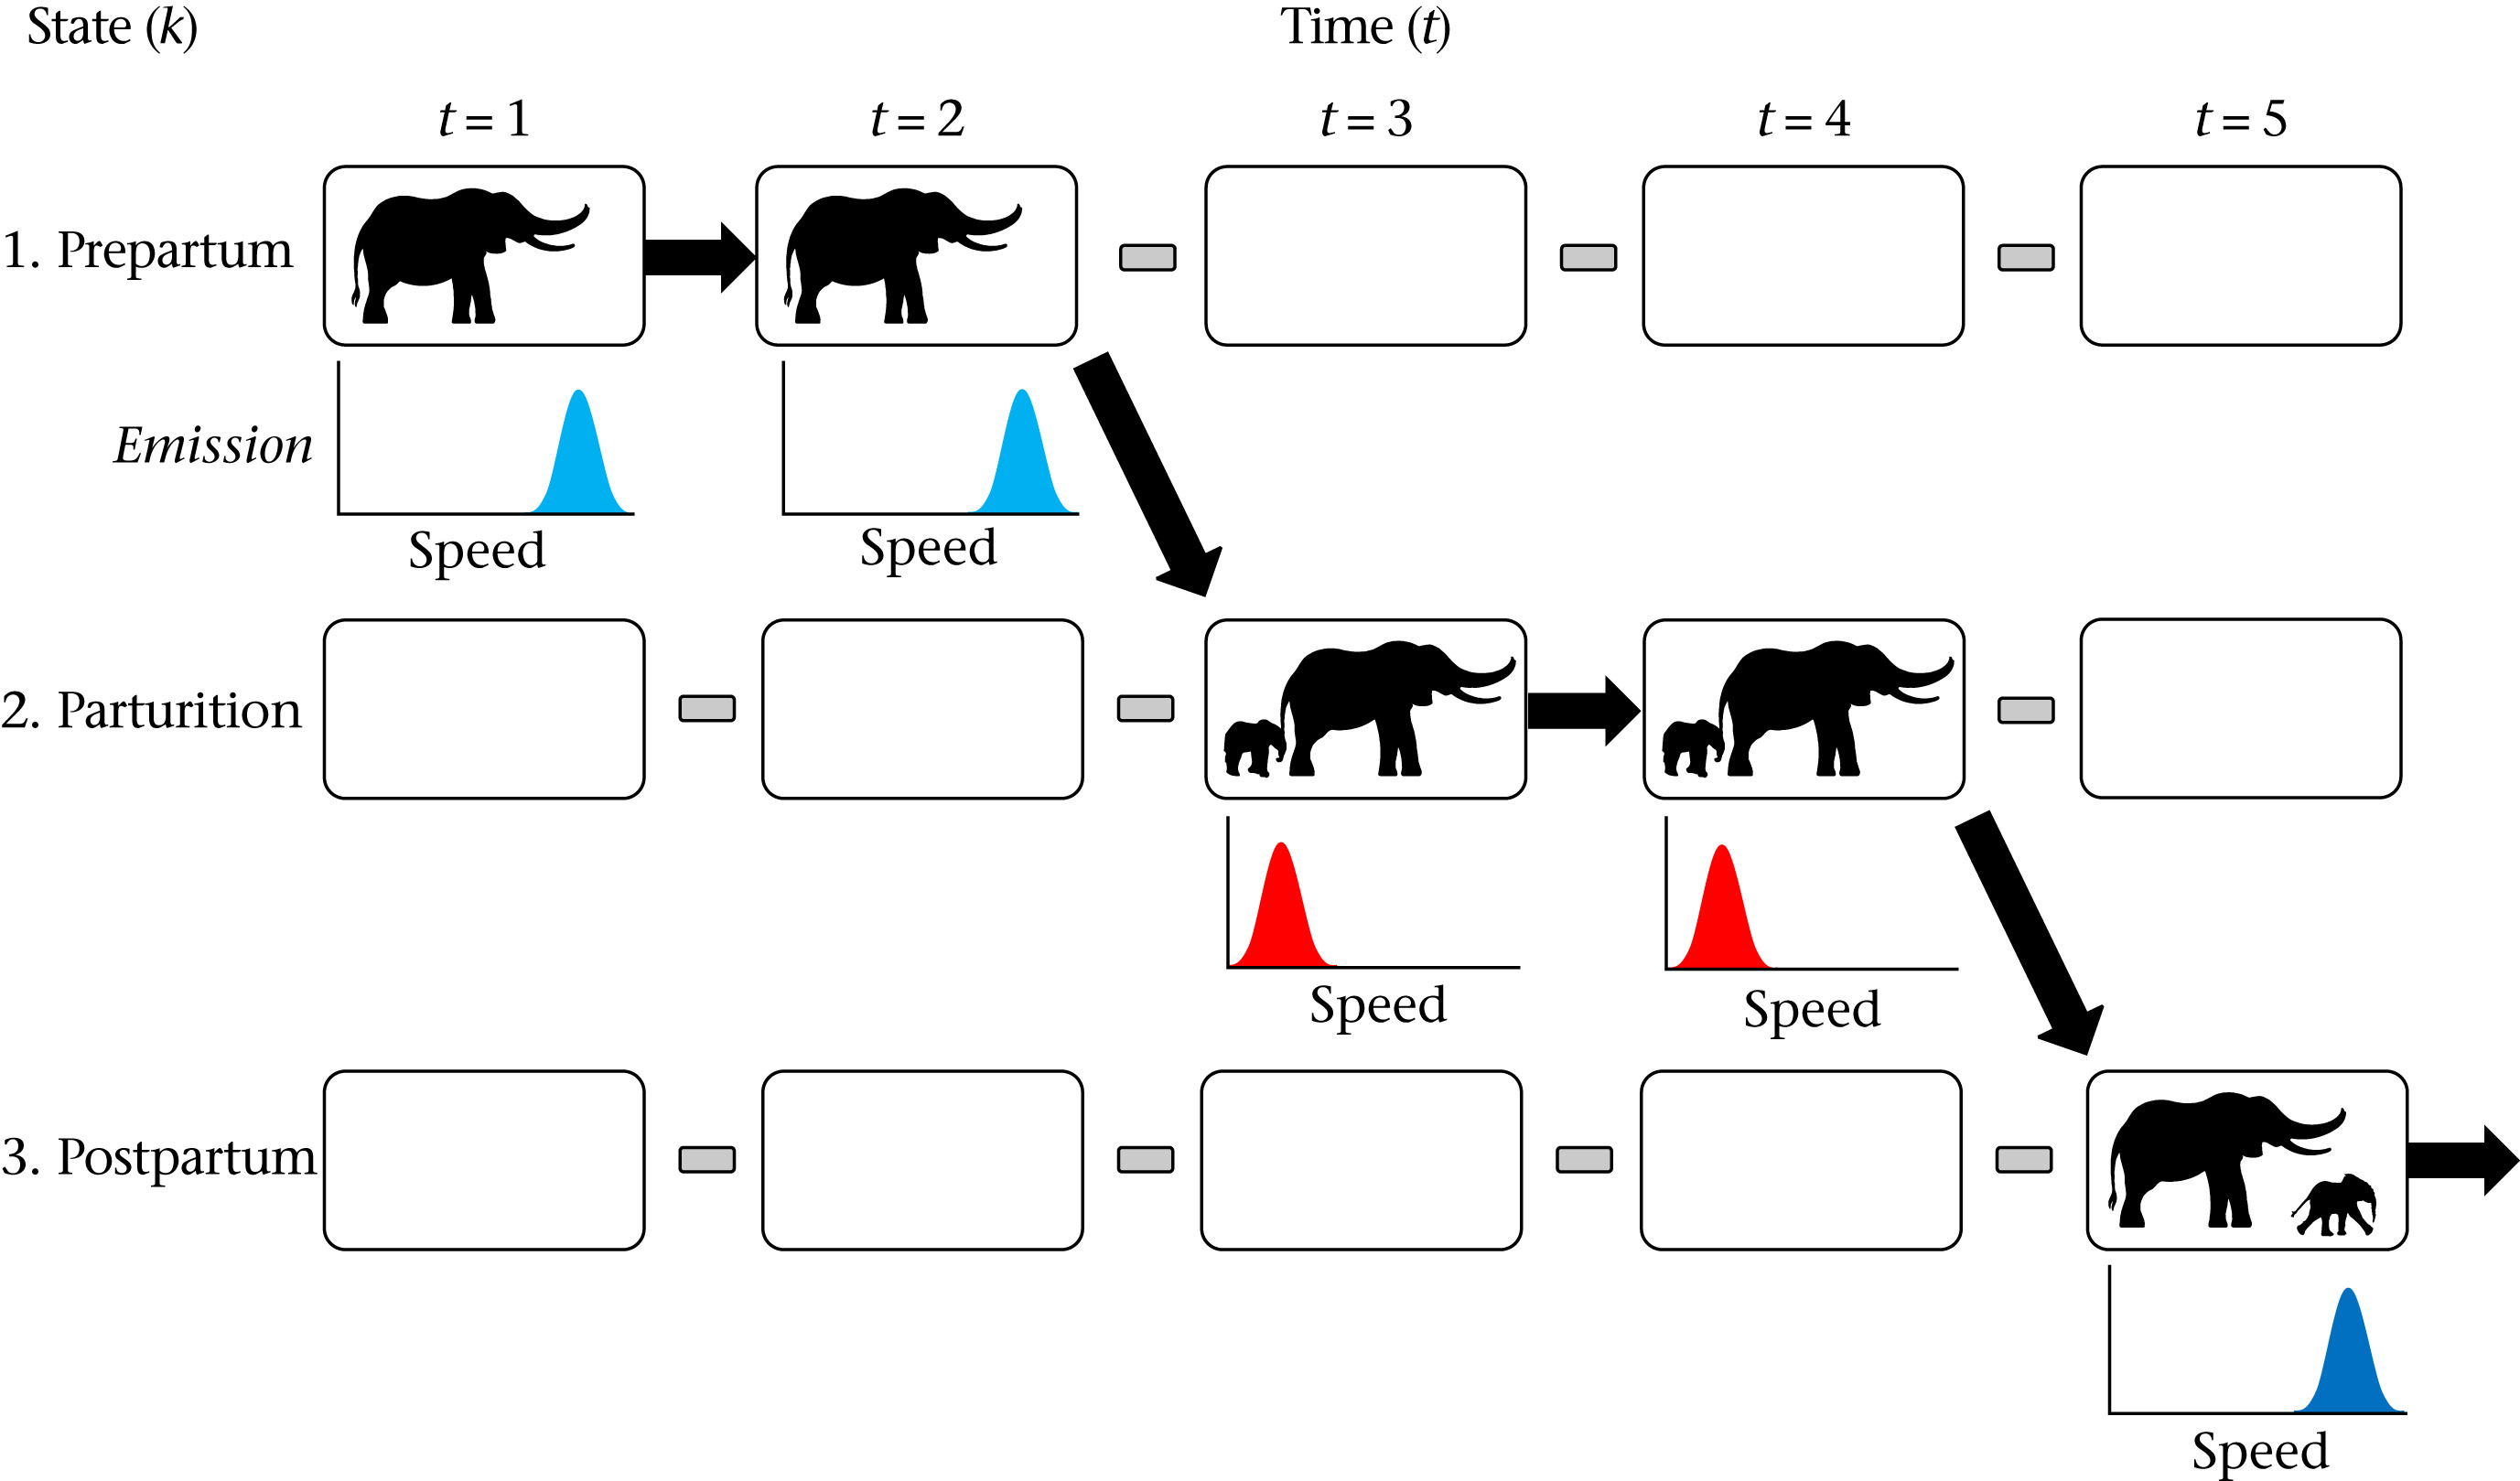
\includegraphics[width=0.8\textwidth]{figures/elephant_parturition.jpg}
    \caption{From Taylor et al. 2022, ``Movement behaviour after birth demonstrates precocial abilities of African savannah elephant, Loxodonta africana, calves''.}
    \label{fig:enter-label}
\end{figure}

\end{frame}

\begin{frame}
\frametitle{Aim of analysis: use data to uncover states and behaviours from imperfect data}

Goals:

\begin{itemize}
    \item Determine an animal state at each point in time
    \item Find an association between states and observations
\end{itemize}
    
\end{frame}

\begin{frame}
\frametitle{Example problem}
Put GPS collars on animals.

Insert GPS figure.
    
\end{frame}

\begin{frame}
\frametitle{Use GPS fixes to determine speed}

\begin{figure}
    \centering
    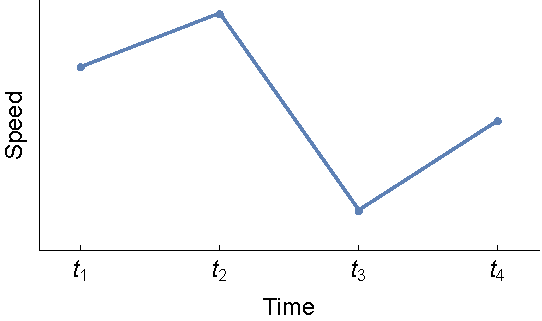
\includegraphics[width=0.8\textwidth]{figures/hmm_time_series.pdf}
\end{figure}
    
\end{frame}

\begin{frame}
\frametitle{An introduction to hidden Markov models (HMMs)}

Let's suppose for simplicity, that an animal can be in one of two behavioural states:

\vspace{0.5cm}

\begin{itemize}
    \item \textit{Migrating} ($m$): animals move directedly at a fast pace
    \item \textit{Foraging} ($f$): animals move slowly as they explore an area
\end{itemize}

\vspace{0.5cm}

Replace with two pictures
    
\end{frame}

\begin{frame}
\frametitle{Emission distributions}
Suppose the animals are collared with GPS machines, allowing us to measure the average animal speed in discrete intervals, $\text{Speed}(xt)$, where $x\in\{m,f\}$.

\vspace{0.5cm}

\begin{itemize}
    \item \textit{Migrating} ($m$): $\text{Speed}(mt)\sim \text{normal}(\theta_m,\sigma_m)$
    \item \textit{Foraging} ($f$): $\text{Speed}(ft)\sim \text{normal}(\theta_f,\sigma_f)$
\end{itemize}

\begin{figure}
    \centering
    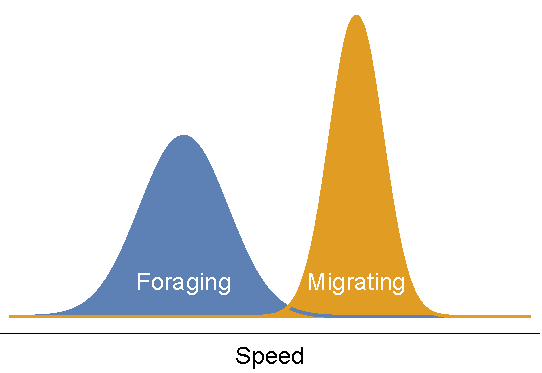
\includegraphics[width=0.55\textwidth]{figures/foraging_migrating.pdf}
\end{figure}
    
\end{frame}

\begin{frame}
\frametitle{A model for how observations are generated}

\begin{center}
\begin{tikzpicture}[node distance=2cm, block/.style={draw, minimum width=1cm, minimum height=1cm}]

  % First row
  \node[block] (A1) {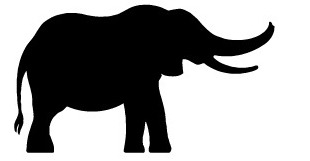
\includegraphics[width=1cm]{figures/elephant.jpg}};
  \node[block, right of=A1] (A2) {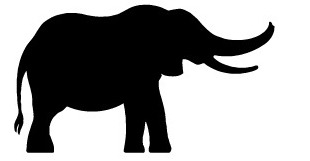
\includegraphics[width=1cm]{figures/elephant.jpg}};
  \node[block, right of=A2] (A3) {};
  \node[block, right of=A3] (A4) {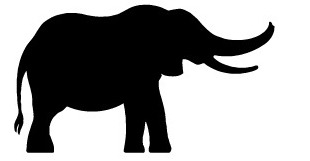
\includegraphics[width=1cm]{figures/elephant.jpg}};

  % Second row
  \node[block, below of=A1] (B1) {};
  \node[block, right of=B1] (B2) {};
  \node[block, right of=B2] (B3) {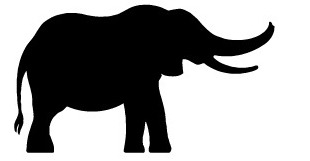
\includegraphics[width=1cm]{figures/elephant.jpg}};
  \node[block, right of=B3] (B4) {};

  % ghost nodes
  \node[coordinate, left of=A1] (J1) {};
  \node[] at (J1) {Migrating:};
  \node[coordinate, left of=B1] (J2) {};
  \node[] at (J2) {Foraging:};
  \node[coordinate, above of=A1, yshift=-0.5cm] (G1) {};
  \node[above] at (G1) {Speed($t_1$)};
  \node[coordinate, above of=A2, yshift=-0.5cm] (G2) {};
  \node[above] at (G2) {Speed($t_2$)};
  \node[coordinate, above of=A3, yshift=-0.5cm] (G3) {};
  \node[coordinate, above of=A4, yshift=-0.5cm] (G4) {};
  \node[above] at (G4) {Speed($t_4$)};
  \node[coordinate, below of=B1, yshift=0.5cm] (H1) {};
  \node[coordinate, below of=B2, yshift=0.5cm] (H2) {};
  \node[coordinate, below of=B3, yshift=0.5cm] (H3) {};
  \node[below] at (H3) {Speed($t_3$)};
  \node[coordinate, below right of=B4] (H4) {};

  % Horizontal arrows
  \draw[->, line width=2pt] (A1.east) -- (A2.west);

  % diagonal to blocks
  \draw[->, line width=2pt] (A2.south east) -- (B3.north);
  \draw[->, line width=2pt] (B3.north east) -- (A4.south);

  % Diagonal arrows
  \draw[->, line width=2pt, orange] (A1.north) -- (G1.west);
  \draw[->, line width=2pt, orange] (A2.north) -- (G2.west);
  \draw[->, line width=2pt, orange] (A4.north) -- (G4.west);
  \draw[->, line width=2pt, blue] (B3.south) -- (H3.west);


  \node[above of=G1,  yshift=-1cm] (timeStart) {};
  \node[above of=G4,  yshift=-1cm] (timeEnd) {};
  \draw[->] (timeStart.west) -- node[above] {Time} (timeEnd.east);

\end{tikzpicture}
\end{center}

\end{frame}

\begin{frame}
\frametitle{The data we actually observe}

\begin{figure}
    \centering
    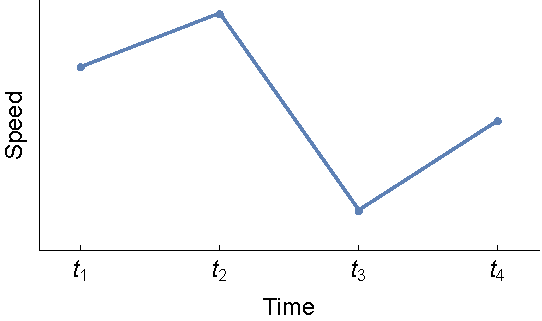
\includegraphics[width=0.8\textwidth]{figures/hmm_time_series.pdf}
\end{figure}
    
\end{frame}

\begin{frame}
\frametitle{The large space of possibilities}

\begin{center}
\begin{tikzpicture}[node distance=2cm, block/.style={draw, minimum width=1cm, minimum height=1cm}]

  % First row
  \node[block] (A1) {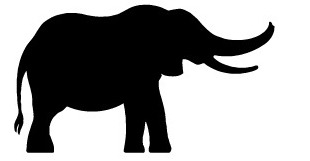
\includegraphics[width=1cm]{figures/elephant.jpg}};
  \node[block, right of=A1] (A2) {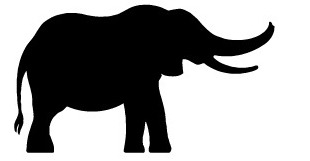
\includegraphics[width=1cm]{figures/elephant.jpg}};
  \node[block, right of=A2] (A3) {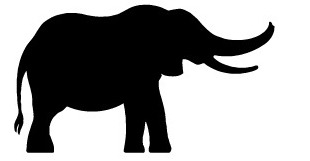
\includegraphics[width=1cm]{figures/elephant.jpg}};
  \node[block, right of=A3] (A4) {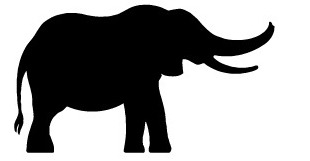
\includegraphics[width=1cm]{figures/elephant.jpg}};

  % Second row
  \node[block, below of=A1] (B1) {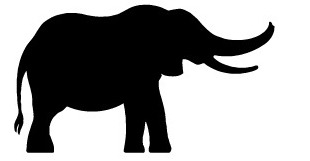
\includegraphics[width=1cm]{figures/elephant.jpg}};
  \node[block, right of=B1] (B2) {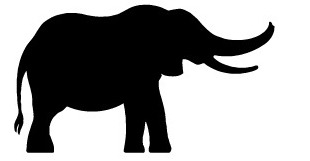
\includegraphics[width=1cm]{figures/elephant.jpg}};
  \node[block, right of=B2] (B3) {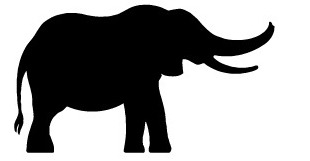
\includegraphics[width=1cm]{figures/elephant.jpg}};
  \node[block, right of=B3] (B4) {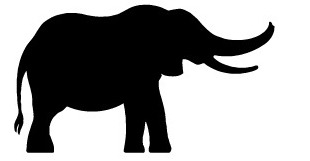
\includegraphics[width=1cm]{figures/elephant.jpg}};

  % ghost nodes
  \node[coordinate, left of=A1] (J1) {};
  \node[] at (J1) {Migrating:};
  \node[coordinate, left of=B1] (J2) {};
  \node[] at (J2) {Foraging:};
  \node[coordinate, above of=A1, yshift=-0.5cm] (G1) {};
  \node[above] at (G1) {Speed($t_1$)};
  \node[coordinate, above of=A2, yshift=-0.5cm] (G2) {};
  \node[above] at (G2) {Speed($t_2$)};
  \node[coordinate, above of=A3, yshift=-0.5cm] (G3) {};
  \node[above] at (G3) {Speed($t_3$)};
  \node[coordinate, above of=A4, yshift=-0.5cm] (G4) {};
  \node[above] at (G4) {Speed($t_4$)};
  \node[coordinate, below of=B1, yshift=0.5cm] (H1) {};
  \node[below] at (H1) {Speed($t_1$)};
  \node[coordinate, below of=B2, yshift=0.5cm] (H2) {};
  \node[below] at (H2) {Speed($t_2$)};
  \node[coordinate, below of=B3, yshift=0.5cm] (H3) {};
  \node[below] at (H3) {Speed($t_3$)};
  \node[coordinate, below of=B4, yshift=0.5cm] (H4) {};
  \node[below] at (H4) {Speed($t_4$)};

  % Horizontal arrows
  \draw[->, line width=2pt] (A1.east) -- (A2.west);
  \draw[->, line width=2pt] (A2.east) -- (A3.west);
  \draw[->, line width=2pt] (A3.east) -- (A4.west);
  \draw[->, line width=2pt] (B1.east) -- (B2.west);
  \draw[->, line width=2pt] (B2.east) -- (B3.west);
  \draw[->, line width=2pt] (B3.east) -- (B4.west);

  % diagonal to blocks
  \draw[->, line width=2pt] (A1.south east) -- (B2.north);
  \draw[->, line width=2pt] (A2.south east) -- (B3.north);
  \draw[->, line width=2pt] (A3.south east) -- (B4.north);
  \draw[->, line width=2pt] (B1.north east) -- (A2.south);
  \draw[->, line width=2pt] (B2.north east) -- (A3.south);
  \draw[->, line width=2pt] (B3.north east) -- (A4.south);

  % vertical arrows
  \draw[->, line width=2pt, orange] (A1.north) -- (G1.west);
  \draw[->, line width=2pt, orange] (A2.north) -- (G2.west);
  \draw[->, line width=2pt, orange] (A3.north) -- (G3.west);
  \draw[->, line width=2pt, orange] (A4.north) -- (G4.west);
  \draw[->, line width=2pt, blue] (B1.south) -- (H1.west);
  \draw[->, line width=2pt, blue] (B2.south) -- (H2.west);
  \draw[->, line width=2pt, blue] (B3.south) -- (H3.west);
  \draw[->, line width=2pt, blue] (B4.south) -- (H4.west);


  \node[above of=G1, yshift=-1cm] (timeStart) {};
  \node[above of=G4, yshift=-1cm] (timeEnd) {};
  \draw[->] (timeStart.west) -- node[above] {Time} (timeEnd.east);

\end{tikzpicture}
\end{center}
    
\end{frame}

\begin{frame}
\frametitle{Start with data}

\begin{center}
\begin{tikzpicture}[node distance=2cm, block/.style={draw, minimum width=1cm, minimum height=1cm}]

  % First row
  \node[block, white] (A1) {};
  \node[block, right of=A1, white] (A2) {};
  \node[block, right of=A2, white] (A3) {};
  \node[block, right of=A3, white] (A4) {};

  % Second row
  \node[block, below of=A1, white] (B1) {};
  \node[block, right of=B1, white] (B2) {};
  \node[block, right of=B2, white] (B3) {};
  \node[block, right of=B3, white] (B4) {};

  % ghost nodes
  \node[coordinate, left of=A1] (J1) {};
  \node[coordinate, left of=B1] (J2) {};
  \node[coordinate, above of=A1, yshift=-0.5cm] (G1) {};
  \node[above] at (G1) {Speed($t_1$)};
  \node[coordinate, above of=A2, yshift=-0.5cm] (G2) {};
  \node[above] at (G2) {Speed($t_2$)};
  \node[coordinate, above of=A3, yshift=-0.5cm] (G3) {};
  \node[above] at (G3) {Speed($t_3$)};
  \node[coordinate, above of=A4, yshift=-0.5cm] (G4) {};
  \node[above] at (G4) {Speed($t_4$)};
  \node[coordinate, below of=B1, yshift=0.5cm] (H1) {};
  \node[coordinate, below of=B2, yshift=0.5cm] (H2) {};
  \node[coordinate, below of=B3, yshift=0.5cm] (H3) {};
  \node[coordinate, below of=B4, yshift=0.5cm] (H4) {};
  \node[below] at (H1) {Speed($t_1$)};
  \node[below] at (H2) {Speed($t_2$)};
  \node[below] at (H3) {Speed($t_3$)};
  \node[below] at (H4) {Speed($t_4$)};


  \node[above of=G1, yshift=-1cm] (timeStart) {};
  \node[above of=G4, yshift=-1cm] (timeEnd) {};
  \draw[->] (timeStart.west) -- node[above] {Time} (timeEnd.east);

\end{tikzpicture}
\end{center}
    
\end{frame}

\begin{frame}
\frametitle{Use data to estimate states and transitions}

\begin{center}
\begin{tikzpicture}[node distance=2cm, block/.style={draw, minimum width=1cm, minimum height=1cm}]

  % First row
  \node[block] (A1) {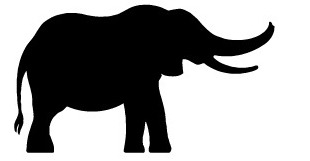
\includegraphics[width=1cm]{figures/elephant.jpg}};
  \node[block, right of=A1] (A2) {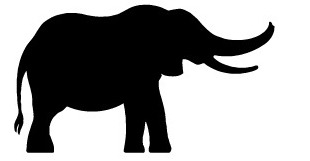
\includegraphics[width=1cm]{figures/elephant.jpg}};
  \node[block, right of=A2] (A3) {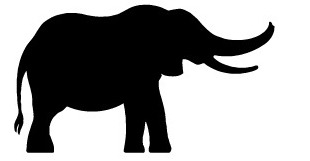
\includegraphics[width=1cm]{figures/elephant.jpg}};
  \node[block, right of=A3] (A4) {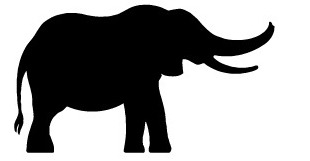
\includegraphics[width=1cm]{figures/elephant.jpg}};

  % Second row
  \node[block, below of=A1] (B1) {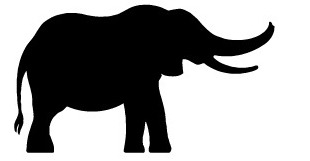
\includegraphics[width=1cm]{figures/elephant.jpg}};
  \node[block, right of=B1] (B2) {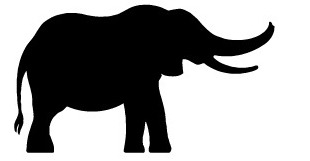
\includegraphics[width=1cm]{figures/elephant.jpg}};
  \node[block, right of=B2] (B3) {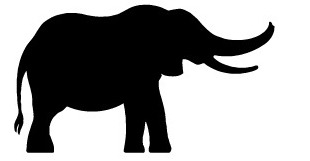
\includegraphics[width=1cm]{figures/elephant.jpg}};
  \node[block, right of=B3] (B4) {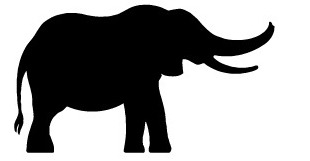
\includegraphics[width=1cm]{figures/elephant.jpg}};
  

  % ghost nodes
  \node[coordinate, left of=A1] (J1) {};
  \node[] at (J1) {Migrating:};
  \node[coordinate, left of=B1] (J2) {};
  \node[] at (J2) {Foraging:};
  \node[coordinate, above of=A1, yshift=-0.5cm] (G1) {};
  \node[above] at (G1) {Speed($t_1$)};
  \node[coordinate, above of=A2, yshift=-0.5cm] (G2) {};
  \node[above] at (G2) {Speed($t_2$)};
  \node[coordinate, above of=A3, yshift=-0.5cm] (G3) {};
  \node[above] at (G3) {Speed($t_3$)};
  \node[coordinate, above of=A4, yshift=-0.5cm] (G4) {};
  \node[above] at (G4) {Speed($t_4$)};
  \node[coordinate, below of=B1, yshift=0.5cm] (H1) {};
  \node[below] at (H1) {Speed($t_1$)};
  \node[coordinate, below of=B2, yshift=0.5cm] (H2) {};
  \node[below] at (H2) {Speed($t_2$)};
  \node[coordinate, below of=B3, yshift=0.5cm] (H3) {};
  \node[below] at (H3) {Speed($t_3$)};
  \node[coordinate, below of=B4, yshift=0.5cm] (H4) {};
  \node[below] at (H4) {Speed($t_4$)};

  % Horizontal arrows
  \draw[->, line width=2pt, opacity=0.5] (A1.east) -- (A2.west);
  \draw[->, line width=2pt, opacity=0.1] (A2.east) -- (A3.west);
  \draw[->, line width=2pt, opacity=0.1] (A3.east) -- (A4.west);
  \draw[->, line width=2pt, opacity=0.1] (B1.east) -- (B2.west);
  \draw[->, line width=2pt, opacity=0.1] (B2.east) -- (B3.west);
  \draw[->, line width=2pt, opacity=0.1] (B3.east) -- (B4.west);

  % diagonal to blocks
  \draw[->, line width=2pt, opacity=0.1] (A1.south east) -- (B2.north);
  \draw[->, line width=2pt, opacity=0.5] (A2.south east) -- (B3.north);
  \draw[->, line width=2pt, opacity=0.1] (A3.south east) -- (B4.north);
  \draw[->, line width=2pt, opacity=0.1] (B1.north east) -- (A2.south);
  \draw[->, line width=2pt, opacity=0.1] (B2.north east) -- (A3.south);
  \draw[->, line width=2pt] (B3.north east) -- (A4.south);

  % vertical arrows
  \draw[<-, line width=2pt, orange] (A1.north) -- (G1.west);
  \draw[<-, line width=2pt, orange] (A2.north) -- (G2.west);
  \draw[<-, line width=2pt, orange] (A3.north) -- (G3.west);
  \draw[<-, line width=2pt, orange] (A4.north) -- (G4.west);
  \draw[<-, line width=2pt, blue] (B1.south) -- (H1.west);
  \draw[<-, line width=2pt, blue] (B2.south) -- (H2.west);
  \draw[<-, line width=2pt, blue] (B3.south) -- (H3.west);
  \draw[<-, line width=2pt, blue] (B4.south) -- (H4.west);


  \node[above of=G1, yshift=-1cm] (timeStart) {};
  \node[above of=G4, yshift=-1cm] (timeEnd) {};
  \draw[->] (timeStart.west) -- node[above] {Time} (timeEnd.east);

\end{tikzpicture}
\end{center}
    
\end{frame}


\begin{frame}
\frametitle{Mathematical description: emission distributions}

\begin{equation}
    \text{Speed}(t, x_t) \overset{\text{iid}}{\sim} \text{normal}(\mu_{x_t}, \sigma_{x_t}),
\end{equation}

where $x[t]\in\{m,f\}$.

\vspace{0.5cm}

This is just a (Gaussian) clustering model.
    
\end{frame}

\begin{frame}
\frametitle{Mathematical description: state transitions}

In HMMs, we typically assume that the state transitions are (1st order) Markovian:
%
\begin{equation}
    p(X_t = a| X_{t-1}, X_{t-2},...,X_0) = p(X_t = a| X_{t-1}),
\end{equation}
%
which means that state transitions can be represented by a $2\times 2$ matrix:
%
\begin{equation}
        \begin{bmatrix} p_{m,m} & p_{m,f}\\ p_{f,m} & p_{f,f} \end{bmatrix} := \begin{bmatrix} p(X_t=m | X_{t-1}=m) & p(X_t=f | X_{t-1}=m) \\ p(X_t=m | X_{t-1}=f) & p(X_t=f | X_{t-1}=f) \end{bmatrix}.
\end{equation}
%
    
\end{frame}

\begin{frame}
\frametitle{Inference problem}

We do not know:

\begin{itemize}
    \item The emission distribution parameters, $\theta := (\mu_f,\mu_m,\sigma_f,\sigma_m),$ 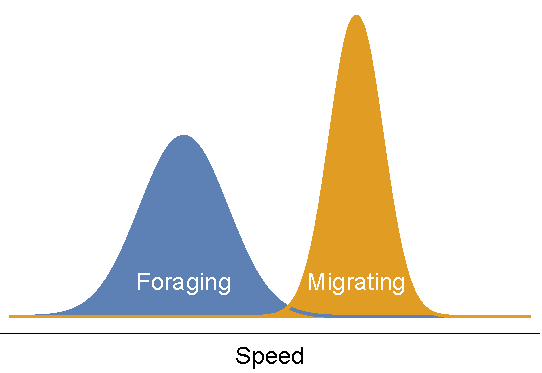
\includegraphics[width=2.5cm]{figures/foraging_migrating.pdf}
    \item The states, \begin{center}
\begin{tikzpicture}[node distance=1cm, block/.style={draw, minimum width=0.5cm, minimum height=0.5cm}]

  % First row
  \node[block] (A1) {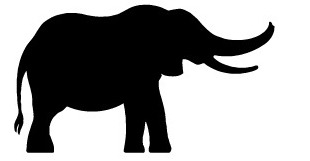
\includegraphics[width=0.5cm]{figures/elephant.jpg}};
  \node[block, right of=A1] (A2) {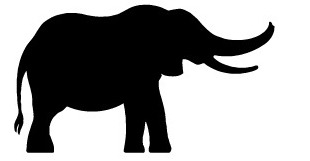
\includegraphics[width=0.5cm]{figures/elephant.jpg}};
  \node[block, right of=A2] (A3) {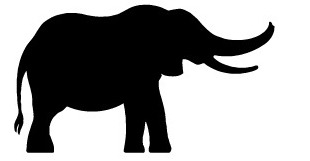
\includegraphics[width=0.5cm]{figures/elephant.jpg}};
  \node[block, right of=A3] (A4) {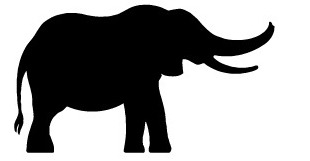
\includegraphics[width=0.5cm]{figures/elephant.jpg}};

  % Second row
  \node[block, below of=A1] (B1) {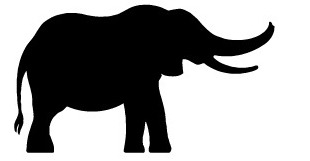
\includegraphics[width=0.5cm]{figures/elephant.jpg}};
  \node[block, right of=B1] (B2) {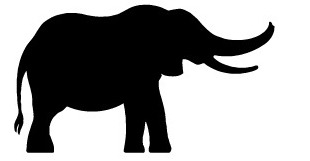
\includegraphics[width=0.5cm]{figures/elephant.jpg}};
  \node[block, right of=B2] (B3) {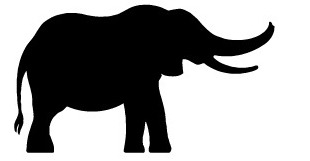
\includegraphics[width=0.5cm]{figures/elephant.jpg}};
  \node[block, right of=B3] (B4) {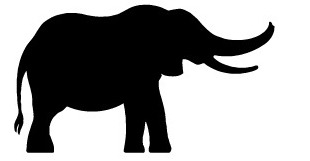
\includegraphics[width=0.5cm]{figures/elephant.jpg}};

  % Horizontal arrows
  \draw[->, line width=1pt, opacity=1] (A1.east) -- (A2.west);
  \draw[->, line width=1pt, opacity=1] (A2.east) -- (A3.west);
  \draw[->, line width=1pt, opacity=1] (A3.east) -- (A4.west);
  \draw[->, line width=1pt, opacity=1] (B1.east) -- (B2.west);
  \draw[->, line width=1pt, opacity=1] (B2.east) -- (B3.west);
  \draw[->, line width=1pt, opacity=1] (B3.east) -- (B4.west);

  % diagonal to blocks
  \draw[->, line width=1pt, opacity=1] (A1.south east) -- (B2.north);
  \draw[->, line width=1pt, opacity=1] (A2.south east) -- (B3.north);
  \draw[->, line width=1pt, opacity=1] (A3.south east) -- (B4.north);
  \draw[->, line width=1pt, opacity=1] (B1.north east) -- (A2.south);
  \draw[->, line width=1pt, opacity=1] (B2.north east) -- (A3.south);
  \draw[->, line width=1pt] (B3.north east) -- (A4.south);

\end{tikzpicture}
\end{center}
\item The transition probability matrix, \begin{equation}
    \begin{bmatrix} p_{m,m} & p_{m,f}\\ p_{f,m} & p_{f,f} \end{bmatrix},
\end{equation}
\end{itemize}

and we want to estimate these from data.
    
\end{frame}

\begin{frame}
\frametitle{Likelihood}

Suppose that we have a list of speeds for a single animal over time: $S:=\{S_t\}_{t=1}^T$.

\vspace{0.5cm}

If we knew the states, $X:=\{X_t\}_{t=1}^T$, since $S_t | X_t \overset{\text{iid}}{\sim} \text{normal}(\mu_{x_t}, \sigma_{x_t})$


the likelihood takes the form:
%
\begin{equation}
    p(S|X,\theta) = \prod_{t=1}^T p(S_t | X_t, \theta).
\end{equation}

But we don't know the states. So what do we do?
    
\end{frame}

\begin{frame}
\frametitle{The joint density of speeds and states}

We consider instead the joint density (suppressing $\theta$ dependence from now on):
%
\begin{equation}
    \begin{aligned}
    p(S, X) &= p(S|X) \times p(X)\\
    &= \left[\prod_{t=1}^T p(S_t | X_t)\right] \times p(X_t)\\
    &= \left[\prod_{t=1}^T p(S_t | X_t)\right] \times \left[\prod_{t=2}^T p(X_t | X_{t-1})\right] p(X_1)
    \end{aligned}
\end{equation}
    
\end{frame}

\begin{frame}
\frametitle{Likelihood revisited}

We can obtain the likelihood by marginalising out $X$ from our joint:
%
\begin{equation}
    p(S) = \sum_X p(S|X) \times p(X).
\end{equation}
%
But this really means:
%
\begin{equation}
    p(S) = \sum_{X_1}\sum_{X_2}...\sum_{X_T}\left[\prod_{t=1}^T p(S_t | X_t)\right] \times \left[\prod_{t=2}^T p(X_t | X_{t-1})\right] p(X_1).
\end{equation}
%
So the computational expense scales as $N^T$, where $N$ is number of states!
    
\end{frame}

\begin{frame}
\frametitle{The forward algorithm: a much cheaper way to evaluate the likelihood}

The \textit{forward algorithm} is an approach from dynamic programming which stores intermediate probabilities.

\vspace{0.5cm}

It uses this trick to calculate the likelihood:

\begin{equation}
    \begin{aligned}
    p(S_1, S_2, ..., S_T) = \sum_{i=1}^N p(S_1, S_2, ..., S_T, X_T=j).
    \end{aligned}
\end{equation}

\vspace{0.5cm}

But how do we calculate the RHS?
    
\end{frame}

\begin{frame}
\frametitle{Forward algorithm bookkeeping}

Consider again the joint distribution of the observations and the final state:

\begin{equation}
    \begin{aligned}
    \textcolor{orange}{p(S_1, S_2, ..., }&\textcolor{orange}{S_T, X_T=j)} = p(S_T | X_T = j) \times\\ &\sum_{i=1}^N p(X_T=j | X_{T-1}=i) \times \textcolor{blue}{p(S_1, S_2, ..., S_{T-1}, X_{T-1}=i)}
    \end{aligned}
\end{equation}

which looks like:

\begin{equation}
    \begin{aligned}
    \textcolor{orange}{\alpha_t(j)} = p(S_T | X_T = j) \times\sum_{i=1}^N p(X_T=j | X_{T-1}=i) \times \textcolor{blue}{\alpha_{t-1}(j)},
    \end{aligned}
\end{equation}

with $\alpha_1(j)=p(S_1 | X_1 = j)p(X_1=j)$.
    
\end{frame}

\begin{frame}
\frametitle{Incremental calculation of likelihood}


\begin{center}
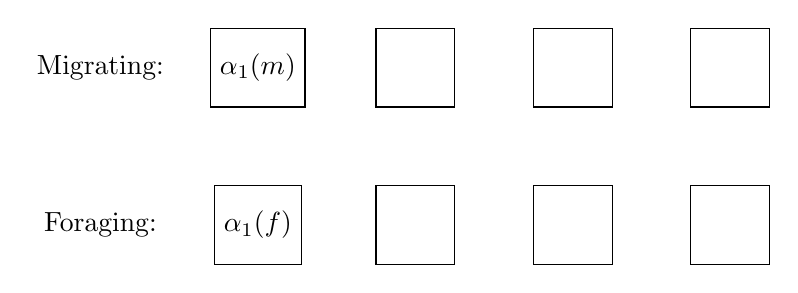
\begin{tikzpicture}[node distance=2cm, block/.style={draw, minimum width=1cm, minimum height=1cm}]

  % First row
  \node[block] (A1) {$\alpha_1(m)$};
  \node[block, right of=A1] (A2) {};
  \node[block, right of=A2] (A3) {};
  \node[block, right of=A3] (A4) {};

  % Second row
  \node[block, below of=A1] (B1) {$\alpha_1(f)$};
  \node[block, right of=B1] (B2) {};
  \node[block, right of=B2] (B3) {};
  \node[block, right of=B3] (B4) {};

  % Labels
  \node[coordinate, left of=A1] (J1) {};
  \node[] at (J1) {Migrating:};
  \node[coordinate, left of=B1] (J2) {};
  \node[] at (J2) {Foraging:};

  % Horizontal arrows
  \draw[->, line width=1pt, opacity=0] (A1.east) -- (A2.west);
  \draw[->, line width=1pt, opacity=0] (A2.east) -- (A3.west);
  \draw[->, line width=1pt, opacity=0] (A3.east) -- (A4.west);
  \draw[->, line width=1pt, opacity=0] (B1.east) -- (B2.west);
  \draw[->, line width=1pt, opacity=0] (B2.east) -- (B3.west);
  \draw[->, line width=1pt, opacity=0] (B3.east) -- (B4.west);

  % diagonal to blocks
  \draw[->, line width=1pt, opacity=0] (A1.south east) -- (B2.north);
  \draw[->, line width=1pt, opacity=0] (A2.south east) -- (B3.north);
  \draw[->, line width=1pt, opacity=0] (A3.south east) -- (B4.north);
  \draw[->, line width=1pt, opacity=0] (B1.north east) -- (A2.south);
  \draw[->, line width=1pt, opacity=0] (B2.north east) -- (A3.south);
  \draw[->, line width=1pt, opacity=0] (B3.north east) -- (A4.south);

\end{tikzpicture}
\end{center}

where $\alpha_1(j)=p(S_1 | X_1 = j)p(X_1=j)$.
    
\end{frame}

\begin{frame}
\frametitle{Incremental calculation of likelihood}


\begin{center}
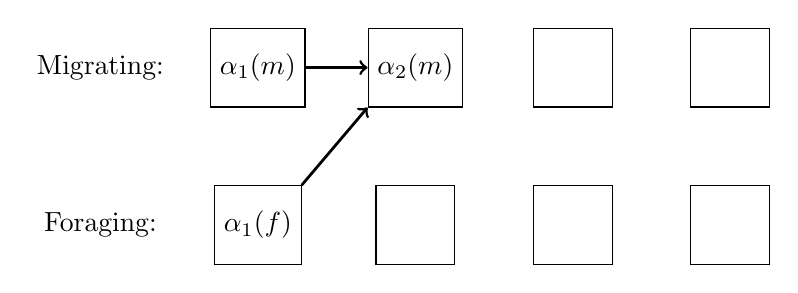
\begin{tikzpicture}[node distance=2cm, block/.style={draw, minimum width=1cm, minimum height=1cm}]

  % First row
  \node[block] (A1) {$\alpha_1(m)$};
  \node[block, right of=A1] (A2) {$\alpha_2(m)$};
  \node[block, right of=A2] (A3) {};
  \node[block, right of=A3] (A4) {};

  % Second row
  \node[block, below of=A1] (B1) {$\alpha_1(f)$};
  \node[block, right of=B1] (B2) {};
  \node[block, right of=B2] (B3) {};
  \node[block, right of=B3] (B4) {};

  % Labels
  \node[coordinate, left of=A1] (J1) {};
  \node[] at (J1) {Migrating:};
  \node[coordinate, left of=B1] (J2) {};
  \node[] at (J2) {Foraging:};

  % Horizontal arrows
  \draw[->, line width=1pt, opacity=1] (A1.east) -- (A2.west);
  \draw[->, line width=1pt, opacity=0] (A2.east) -- (A3.west);
  \draw[->, line width=1pt, opacity=0] (A3.east) -- (A4.west);
  \draw[->, line width=1pt, opacity=0] (B1.east) -- (B2.west);
  \draw[->, line width=1pt, opacity=0] (B2.east) -- (B3.west);
  \draw[->, line width=1pt, opacity=0] (B3.east) -- (B4.west);

  % diagonal to blocks
  \draw[->, line width=1pt, opacity=0] (A1.south east) -- (B2.north);
  \draw[->, line width=1pt, opacity=0] (A2.south east) -- (B3.north);
  \draw[->, line width=1pt, opacity=0] (A3.south east) -- (B4.north);
  \draw[->, line width=1pt, opacity=1] (B1.north east) -- (A2.south west);
  \draw[->, line width=1pt, opacity=0] (B2.north east) -- (A3.south);
  \draw[->, line width=1pt, opacity=0] (B3.north east) -- (A4.south);

\end{tikzpicture}
\end{center}

where: 
\begin{equation}
    \begin{aligned}
    \alpha_2(m) = p(&S_2 | X_2 = m) \times\\
    &\{p(X_2=m | X_1=m) \alpha_{1}(m) +p(X_2=m | X_1=f) \alpha_{1}(f)\}.
    \end{aligned}
\end{equation}
    
\end{frame}

\begin{frame}
\frametitle{Incremental calculation of likelihood}


\begin{center}
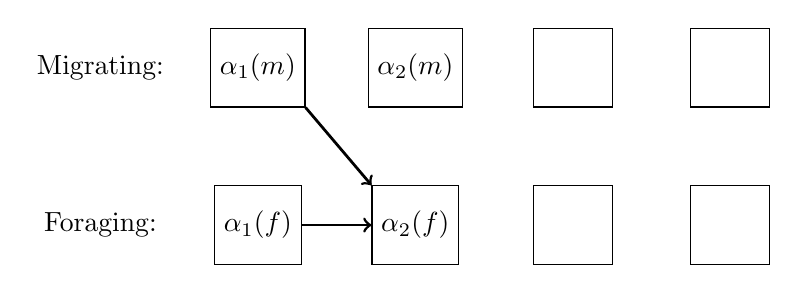
\begin{tikzpicture}[node distance=2cm, block/.style={draw, minimum width=1cm, minimum height=1cm}]

  % First row
  \node[block] (A1) {$\alpha_1(m)$};
  \node[block, right of=A1] (A2) {$\alpha_2(m)$};
  \node[block, right of=A2] (A3) {};
  \node[block, right of=A3] (A4) {};

  % Second row
  \node[block, below of=A1] (B1) {$\alpha_1(f)$};
  \node[block, right of=B1] (B2) {$\alpha_2(f)$};
  \node[block, right of=B2] (B3) {};
  \node[block, right of=B3] (B4) {};

  % Labels
  \node[coordinate, left of=A1] (J1) {};
  \node[] at (J1) {Migrating:};
  \node[coordinate, left of=B1] (J2) {};
  \node[] at (J2) {Foraging:};

  % Horizontal arrows
  \draw[->, line width=1pt, opacity=0] (A1.east) -- (A2.west);
  \draw[->, line width=1pt, opacity=0] (A2.east) -- (A3.west);
  \draw[->, line width=1pt, opacity=0] (A3.east) -- (A4.west);
  \draw[->, line width=1pt, opacity=1] (B1.east) -- (B2.west);
  \draw[->, line width=1pt, opacity=0] (B2.east) -- (B3.west);
  \draw[->, line width=1pt, opacity=0] (B3.east) -- (B4.west);

  % diagonal to blocks
  \draw[->, line width=1pt, opacity=1] (A1.south east) -- (B2.north west);
  \draw[->, line width=1pt, opacity=0] (A2.south east) -- (B3.north);
  \draw[->, line width=1pt, opacity=0] (A3.south east) -- (B4.north);
  \draw[->, line width=1pt, opacity=0] (B1.north east) -- (A2.south west);
  \draw[->, line width=1pt, opacity=0] (B2.north east) -- (A3.south);
  \draw[->, line width=1pt, opacity=0] (B3.north east) -- (A4.south);

\end{tikzpicture}
\end{center}

where: 
\begin{equation}
    \begin{aligned}
    \alpha_2(f) = p(&S_2| X_2 = f) \times \\
    &\{p(X_2=f | X_1=m) \alpha_{1}(m) +p(X_2=f | X_1=f) \alpha_{1}(f)\}.
    \end{aligned}
\end{equation}
    
\end{frame}

\begin{frame}
\frametitle{Incremental calculation of likelihood}


\begin{center}
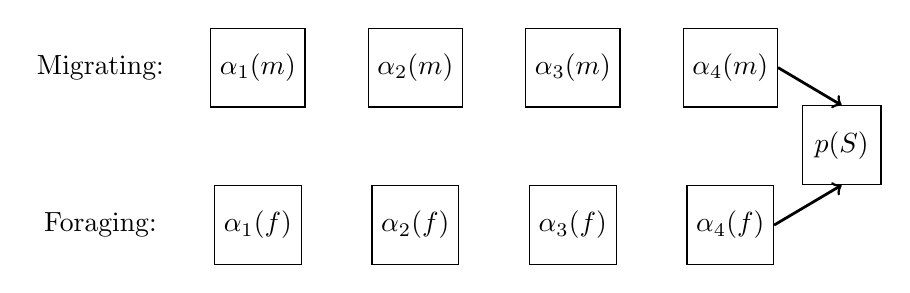
\begin{tikzpicture}[node distance=2cm, block/.style={draw, minimum width=1cm, minimum height=1cm}]

  % First row
  \node[block] (A1) {$\alpha_1(m)$};
  \node[block, right of=A1] (A2) {$\alpha_2(m)$};
  \node[block, right of=A2] (A3) {$\alpha_3(m)$};
  \node[block, right of=A3] (A4) {$\alpha_4(m)$};

  % Second row
  \node[block, below of=A1] (B1) {$\alpha_1(f)$};
  \node[block, right of=B1] (B2) {$\alpha_2(f)$};
  \node[block, right of=B2] (B3) {$\alpha_3(f)$};
  \node[block, right of=B3] (B4) {$\alpha_4(f)$};


  % Labels
  \node[coordinate, left of=A1] (J1) {};
  \node[] at (J1) {Migrating:};
  \node[coordinate, left of=B1] (J2) {};
  \node[] at (J2) {Foraging:};

  % Horizontal arrows
  \draw[->, line width=1pt, opacity=0] (A1.east) -- (A2.west);
  \draw[->, line width=1pt, opacity=0] (A2.east) -- (A3.west);
  \draw[->, line width=1pt, opacity=0] (A3.east) -- (A4.west);
  \draw[->, line width=1pt, opacity=0] (B1.east) -- (B2.west);
  \draw[->, line width=1pt, opacity=0] (B2.east) -- (B3.west);
  \draw[->, line width=1pt, opacity=0] (B3.east) -- (B4.west);

  % diagonal to blocks
  \draw[->, line width=1pt, opacity=0] (A1.south east) -- (B2.north west);
  \draw[->, line width=1pt, opacity=0] (A2.south east) -- (B3.north);
  \draw[->, line width=1pt, opacity=0] (A3.south east) -- (B4.north);
  \draw[->, line width=1pt, opacity=0] (B1.north east) -- (A2.south west);
  \draw[->, line width=1pt, opacity=0] (B2.north east) -- (A3.south);
  \draw[->, line width=1pt, opacity=0] (B3.north east) -- (A4.south);

  \node[block, above right of=B4, yshift=-0.4cm] (C1) {$p(S)$};
  \draw[->, line width=1pt, opacity=1] (B4.east) -- (C1.south);
  \draw[->, line width=1pt, opacity=1] (A4.east) -- (C1.north);

\end{tikzpicture}
\end{center}

and calculate likelihood via:
%
\begin{equation}
    \begin{aligned}
        p(S) = \alpha_4(m) + \alpha_4(f).
    \end{aligned}
\end{equation}
    
\end{frame}

\begin{frame}
\frametitle{Computational expense of forward algorithm}

\begin{itemize}
    \item Naive approach: $O(N^T)$
    \item Forward algorithm: $O(N^2 T)$
\end{itemize}
    
\end{frame}

\begin{frame}
\frametitle{Estimating the states}

The forward algorithm calculates $p(S)$ by marginalising the state vector $X$ out of the joint distribution $p(S,X)$.

\vspace{0.5cm}

But how do we estimate the state? One criterion is to choose the states, $X_1,X_2,...,X_T$ such that:

\vspace{0.5cm}

\begin{equation}
    X_1, X_2, ..., X_T = \argmax_{X_1, X_2, ..., X_T}{p(X_1,X_2,...,X_T,S_1, S_2,...,S_T)}
\end{equation}

\vspace{0.5cm}

But a brute force search is $O(N^T)$!

\end{frame}

\begin{frame}
\frametitle{The Viterbi algorithm}

Instead, we use a dynamic programming algorithm called the \textit{Viterbi} algorithm.

\vspace{0.5cm}

Starts at the beginning of the time series, and, in each subsequent time, it calculates:
%
\begin{equation}
    v_t(i) = \max_{X_1, X_2, ..., X_{t-1}} p(X_1, X_2, ..., X_{t-1}, X_t=i, S_1, S_2, ..., S_{t-1}, S_t).
\end{equation}
%
This can be calculated recursively as:
%
\begin{equation}
    v_t(i) = \left[\max_{j} v_{t-1}(j) p(X_t=i|X_{t-1}=j)\right] p(S_t|X_t=i).
\end{equation}
%
We also record which path lead us here:
%
\begin{equation}
    \psi_t(i) = \argmax_{j} v_{t-1}(j) p(X_t=i|X_{t-1}=j).
\end{equation}
    
\end{frame}

\begin{frame}
\frametitle{Viterbi in action}

\begin{center}
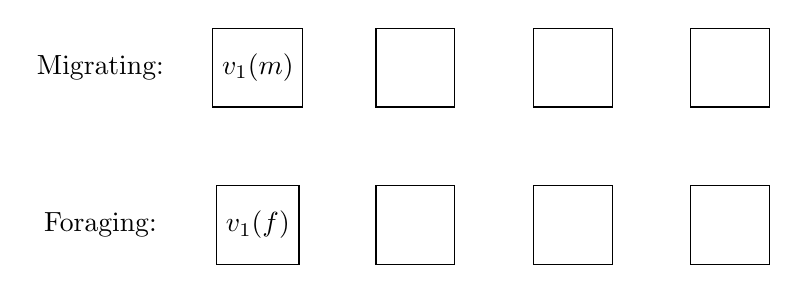
\begin{tikzpicture}[node distance=2cm, block/.style={draw, minimum width=1cm, minimum height=1cm}]

  % First row
  \node[block] (A1) {$v_1(m)$};
  \node[block, right of=A1] (A2) {};
  \node[block, right of=A2] (A3) {};
  \node[block, right of=A3] (A4) {};

  % Second row
  \node[block, below of=A1] (B1) {$v_1(f)$};
  \node[block, right of=B1] (B2) {};
  \node[block, right of=B2] (B3) {};
  \node[block, right of=B3] (B4) {};

  % Labels
  \node[coordinate, left of=A1] (J1) {};
  \node[] at (J1) {Migrating:};
  \node[coordinate, left of=B1] (J2) {};
  \node[] at (J2) {Foraging:};

  % Horizontal arrows
  \draw[->, line width=1pt, opacity=0] (A1.east) -- (A2.west);
  \draw[->, line width=1pt, opacity=0] (A2.east) -- (A3.west);
  \draw[->, line width=1pt, opacity=0] (A3.east) -- (A4.west);
  \draw[->, line width=1pt, opacity=0] (B1.east) -- (B2.west);
  \draw[->, line width=1pt, opacity=0] (B2.east) -- (B3.west);
  \draw[->, line width=1pt, opacity=0] (B3.east) -- (B4.west);

  % diagonal to blocks
  \draw[->, line width=1pt, opacity=0] (A1.south east) -- (B2.north);
  \draw[->, line width=1pt, opacity=0] (A2.south east) -- (B3.north);
  \draw[->, line width=1pt, opacity=0] (A3.south east) -- (B4.north);
  \draw[->, line width=1pt, opacity=0] (B1.north east) -- (A2.south);
  \draw[->, line width=1pt, opacity=0] (B2.north east) -- (A3.south);
  \draw[->, line width=1pt, opacity=0] (B3.north east) -- (A4.south);

\end{tikzpicture}
\end{center}

where $v_1(j) = p(S_1|X_1=j)p(X_1=j)$.
    
\end{frame}

\begin{frame}
\frametitle{Viterbi in action}

\begin{center}
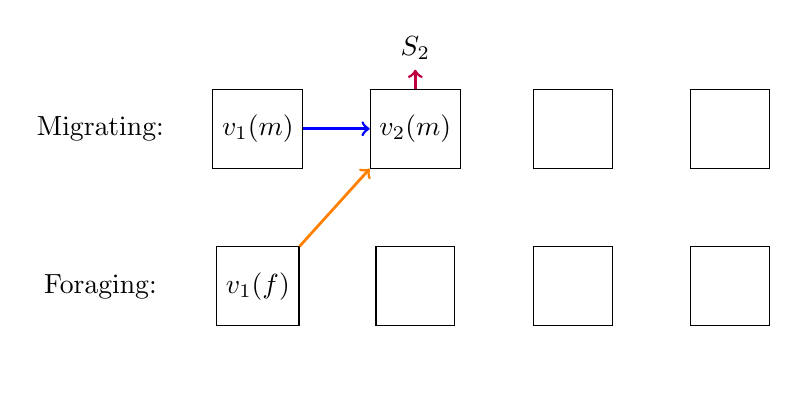
\begin{tikzpicture}[node distance=2cm, block/.style={draw, minimum width=1cm, minimum height=1cm}]

  % First row
  \node[block] (A1) {$v_1(m)$};
  \node[block, right of=A1] (A2) {$v_2(m)$};
  \node[block, right of=A2] (A3) {};
  \node[block, right of=A3] (A4) {};

  % Second row
  \node[block, below of=A1] (B1) {$v_1(f)$};
  \node[block, right of=B1] (B2) {};
  \node[block, right of=B2] (B3) {};
  \node[block, right of=B3] (B4) {};

  % Labels
  \node[coordinate, left of=A1] (J1) {};
  \node[] at (J1) {Migrating:};
  \node[coordinate, left of=B1] (J2) {};
  \node[] at (J2) {Foraging:};

  % Horizontal arrows
  \draw[->, line width=1pt, opacity=1, color=blue] (A1.east) -- (A2.west);
  \draw[->, line width=1pt, opacity=0] (A2.east) -- (A3.west);
  \draw[->, line width=1pt, opacity=0] (A3.east) -- (A4.west);
  \draw[->, line width=1pt, opacity=0] (B1.east) -- (B2.west);
  \draw[->, line width=1pt, opacity=0] (B2.east) -- (B3.west);
  \draw[->, line width=1pt, opacity=0] (B3.east) -- (B4.west);

  % diagonal to blocks
  \draw[->, line width=1pt, opacity=0] (A1.south east) -- (B2.north);
  \draw[->, line width=1pt, opacity=0] (A2.south east) -- (B3.north);
  \draw[->, line width=1pt, opacity=0] (A3.south east) -- (B4.north);
  \draw[->, line width=1pt, opacity=1, color=orange] (B1.north east) -- (A2.south west);
  \draw[->, line width=1pt, opacity=0] (B2.north east) -- (A3.south);
  \draw[->, line width=1pt, opacity=0] (B3.north east) -- (A4.south);

  \node[coordinate, above of=A1, yshift=-1.25cm] (G1) {};
  \node[above] at (G1) {};
  \node[coordinate, above of=A2, yshift=-1.25cm] (G2) {};
  \node[above] at (G2) {$S_2$};
  \node[coordinate, above of=A3, yshift=-1.25cm] (G3) {};
  \node[above] at (G3) {};
  \node[coordinate, above of=A4, yshift=-1.25cm] (G4) {};
  \node[above] at (G4) {};
  \node[coordinate, below of=B1, yshift=1.25cm] (H1) {};
  \node[below] at (H1) {};
  \node[coordinate, below of=B2, yshift=1.25cm] (H2) {};
  \node[below] at (H2) {};
  \node[coordinate, below of=B3, yshift=1.25cm] (H3) {};
  \node[below] at (H3) {};
  \node[coordinate, below of=B4, yshift=1.25cm] (H4) {};
  \node[below] at (H4) {};

  % vertical arrow
  \draw[->, line width=1pt, opacity=1, color=purple] (A2.north) -- (G2.south);

\end{tikzpicture}
\end{center}


\begin{equation*}
\begin{aligned}
    v_2(m) = \max\{&\textcolor{blue}{v_1(m) p(X_2=m | X_1=m)}, \textcolor{orange}{v_1(f) p(X_2=m | X_1=f)} \} \times\\
    &\textcolor{purple}{p(S_2|X_2=m)}.
\end{aligned}
\end{equation*}
    
\end{frame}

\begin{frame}
\frametitle{Viterbi in action}
\begin{center}
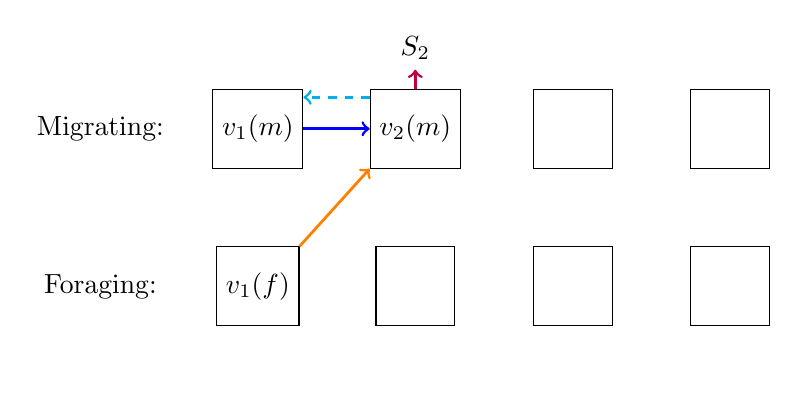
\begin{tikzpicture}[node distance=2cm, block/.style={draw, minimum width=1cm, minimum height=1cm}]

  % First row
  \node[block] (A1) {$v_1(m)$};
  \node[block, right of=A1] (A2) {$v_2(m)$};
  \node[block, right of=A2] (A3) {};
  \node[block, right of=A3] (A4) {};

  % Second row
  \node[block, below of=A1] (B1) {$v_1(f)$};
  \node[block, right of=B1] (B2) {};
  \node[block, right of=B2] (B3) {};
  \node[block, right of=B3] (B4) {};

  % Labels
  \node[coordinate, left of=A1] (J1) {};
  \node[] at (J1) {Migrating:};
  \node[coordinate, left of=B1] (J2) {};
  \node[] at (J2) {Foraging:};

  % Horizontal arrows
  \draw[->, line width=1pt, opacity=1, color=blue] (A1.east) -- (A2.west);
  \draw[->, line width=1pt, opacity=0] (A2.east) -- (A3.west);
  \draw[->, line width=1pt, opacity=0] (A3.east) -- (A4.west);
  \draw[->, line width=1pt, opacity=0] (B1.east) -- (B2.west);
  \draw[->, line width=1pt, opacity=0] (B2.east) -- (B3.west);
  \draw[->, line width=1pt, opacity=0] (B3.east) -- (B4.west);

  % Horizontal back-pointers
  \draw[->, line width=1pt, opacity=1, color=cyan, dashed] ($(A2.west)+(0,0.4cm)$) -- ($(A1.east)+(0,0.4cm)$);

  % diagonal to blocks
  \draw[->, line width=1pt, opacity=0] (A1.south east) -- (B2.north);
  \draw[->, line width=1pt, opacity=0] (A2.south east) -- (B3.north);
  \draw[->, line width=1pt, opacity=0] (A3.south east) -- (B4.north);
  \draw[->, line width=1pt, opacity=1, color=orange] (B1.north east) -- (A2.south west);
  \draw[->, line width=1pt, opacity=0] (B2.north east) -- (A3.south);
  \draw[->, line width=1pt, opacity=0] (B3.north east) -- (A4.south);

  \node[coordinate, above of=A1, yshift=-1.25cm] (G1) {};
  \node[above] at (G1) {};
  \node[coordinate, above of=A2, yshift=-1.25cm] (G2) {};
  \node[above] at (G2) {$S_2$};
  \node[coordinate, above of=A3, yshift=-1.25cm] (G3) {};
  \node[above] at (G3) {};
  \node[coordinate, above of=A4, yshift=-1.25cm] (G4) {};
  \node[above] at (G4) {};
  \node[coordinate, below of=B1, yshift=1.25cm] (H1) {};
  \node[below] at (H1) {};
  \node[coordinate, below of=B2, yshift=1.25cm] (H2) {};
  \node[below] at (H2) {};
  \node[coordinate, below of=B3, yshift=1.25cm] (H3) {};
  \node[below] at (H3) {};
  \node[coordinate, below of=B4, yshift=1.25cm] (H4) {};
  \node[below] at (H4) {};

  % vertical arrow
  \draw[->, line width=1pt, opacity=1, color=purple] (A2.north) -- (G2.south);

\end{tikzpicture}
\end{center}


\begin{equation*}
    \text{if } \textcolor{blue}{v_1(m) p(X_2=m | X_1=m)} > \textcolor{orange}{v_1(f) p(X_2=m | X_1=f)}
\end{equation*}
    
\end{frame}

\begin{frame}
\frametitle{Viterbi in action}
\begin{center}
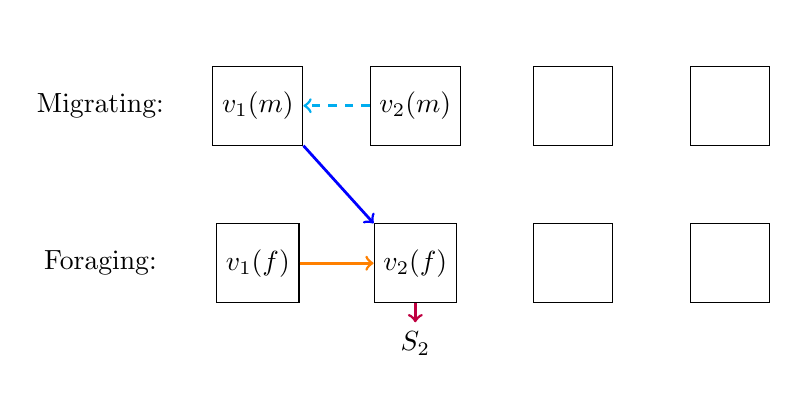
\begin{tikzpicture}[node distance=2cm, block/.style={draw, minimum width=1cm, minimum height=1cm}]

  % First row
  \node[block] (A1) {$v_1(m)$};
  \node[block, right of=A1] (A2) {$v_2(m)$};
  \node[block, right of=A2] (A3) {};
  \node[block, right of=A3] (A4) {};

  % Second row
  \node[block, below of=A1] (B1) {$v_1(f)$};
  \node[block, right of=B1] (B2) {$v_2(f)$};
  \node[block, right of=B2] (B3) {};
  \node[block, right of=B3] (B4) {};

  % Labels
  \node[coordinate, left of=A1] (J1) {};
  \node[] at (J1) {Migrating:};
  \node[coordinate, left of=B1] (J2) {};
  \node[] at (J2) {Foraging:};

  % Horizontal arrows
  \draw[->, line width=1pt, opacity=0, color=blue] (A1.east) -- (A2.west);
  \draw[->, line width=1pt, opacity=1, color=cyan, dashed] (A2.west) -- (A1.east);
  \draw[->, line width=1pt, opacity=0] (A3.east) -- (A4.west);
  \draw[->, line width=1pt, opacity=1, color=orange] (B1.east) -- (B2.west);
  \draw[->, line width=1pt, opacity=0] (B2.east) -- (B3.west);
  \draw[->, line width=1pt, opacity=0] (B3.east) -- (B4.west);

  % diagonal to blocks
  \draw[->, line width=1pt, opacity=1, color=blue] (A1.south east) -- (B2.north west);
  \draw[->, line width=1pt, opacity=0] (A2.south east) -- (B3.north);
  \draw[->, line width=1pt, opacity=0] (A3.south east) -- (B4.north);
  \draw[->, line width=1pt, opacity=0, color=orange] (B1.north east) -- (A2.south west);
  \draw[->, line width=1pt, opacity=0] (B2.north east) -- (A3.south);
  \draw[->, line width=1pt, opacity=0] (B3.north east) -- (A4.south);

  \node[coordinate, above of=A1, yshift=-1.25cm] (G1) {};
  \node[above] at (G1) {};
  \node[coordinate, above of=A2, yshift=-1.25cm] (G2) {};
  \node[above] at (G2) {};
  \node[coordinate, above of=A3, yshift=-1.25cm] (G3) {};
  \node[above] at (G3) {};
  \node[coordinate, above of=A4, yshift=-1.25cm] (G4) {};
  \node[above] at (G4) {};
  \node[coordinate, below of=B1, yshift=1.25cm] (H1) {};
  \node[below] at (H1) {};
  \node[coordinate, below of=B2, yshift=1.25cm] (H2) {};
  \node[below] at (H2) {$S_2$};
  \node[coordinate, below of=B3, yshift=1.25cm] (H3) {};
  \node[below] at (H3) {};
  \node[coordinate, below of=B4, yshift=1.25cm] (H4) {};
  \node[below] at (H4) {};

  % vertical arrow
  \draw[->, line width=1pt, opacity=1, color=purple] (B2.south) -- (H2.north);

\end{tikzpicture}
\end{center}


\begin{equation*}
\begin{aligned}
    v_2(f) = \max\{&\textcolor{blue}{v_1(m) p(X_2=f | X_1=m)}, \textcolor{orange}{v_1(f) p(X_2=f | X_1=f)} \} \times\\
    &\textcolor{purple}{p(S_2|X_2=f)}.
\end{aligned}
\end{equation*}
    
\end{frame}

\begin{frame}
\frametitle{Viterbi in action}
\begin{center}
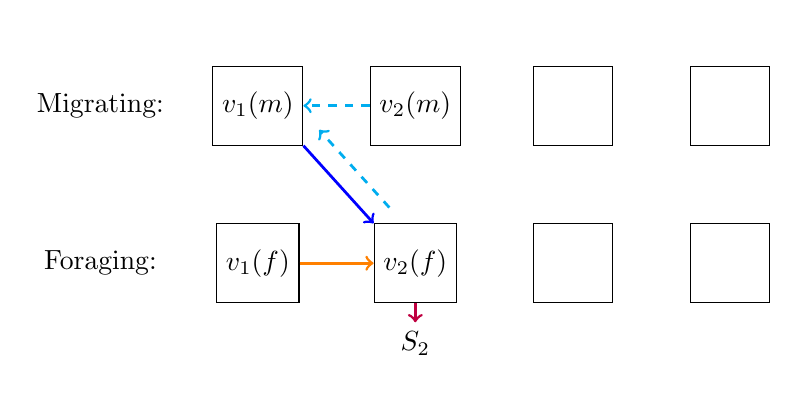
\begin{tikzpicture}[node distance=2cm, block/.style={draw, minimum width=1cm, minimum height=1cm}]

  % First row
  \node[block] (A1) {$v_1(m)$};
  \node[block, right of=A1] (A2) {$v_2(m)$};
  \node[block, right of=A2] (A3) {};
  \node[block, right of=A3] (A4) {};

  % Second row
  \node[block, below of=A1] (B1) {$v_1(f)$};
  \node[block, right of=B1] (B2) {$v_2(f)$};
  \node[block, right of=B2] (B3) {};
  \node[block, right of=B3] (B4) {};

  % Labels
  \node[coordinate, left of=A1] (J1) {};
  \node[] at (J1) {Migrating:};
  \node[coordinate, left of=B1] (J2) {};
  \node[] at (J2) {Foraging:};

  % Horizontal arrows
  \draw[->, line width=1pt, opacity=0, color=blue] (A1.east) -- (A2.west);
  \draw[->, line width=1pt, opacity=1, color=cyan, dashed] (A2.west) -- (A1.east);
  \draw[->, line width=1pt, opacity=0] (A3.east) -- (A4.west);
  \draw[->, line width=1pt, opacity=1, color=orange] (B1.east) -- (B2.west);
  \draw[->, line width=1pt, opacity=0] (B2.east) -- (B3.west);
  \draw[->, line width=1pt, opacity=0] (B3.east) -- (B4.west);

  % Back-pointers
  \draw[->, line width=1pt, opacity=1, color=cyan, dashed] ($(B2.north west)+(0.2cm,0.2cm)$) -- ($(A1.south east)+(0.2cm,0.2cm)$);
  

  % diagonal to blocks
  \draw[->, line width=1pt, opacity=1, color=blue] (A1.south east) -- (B2.north west);
  \draw[->, line width=1pt, opacity=0] (A2.south east) -- (B3.north);
  \draw[->, line width=1pt, opacity=0] (A3.south east) -- (B4.north);
  \draw[->, line width=1pt, opacity=0, color=orange] (B1.north east) -- (A2.south west);
  \draw[->, line width=1pt, opacity=0] (B2.north east) -- (A3.south);
  \draw[->, line width=1pt, opacity=0] (B3.north east) -- (A4.south);

  \node[coordinate, above of=A1, yshift=-1.25cm] (G1) {};
  \node[above] at (G1) {};
  \node[coordinate, above of=A2, yshift=-1.25cm] (G2) {};
  \node[above] at (G2) {};
  \node[coordinate, above of=A3, yshift=-1.25cm] (G3) {};
  \node[above] at (G3) {};
  \node[coordinate, above of=A4, yshift=-1.25cm] (G4) {};
  \node[above] at (G4) {};
  \node[coordinate, below of=B1, yshift=1.25cm] (H1) {};
  \node[below] at (H1) {};
  \node[coordinate, below of=B2, yshift=1.25cm] (H2) {};
  \node[below] at (H2) {$S_2$};
  \node[coordinate, below of=B3, yshift=1.25cm] (H3) {};
  \node[below] at (H3) {};
  \node[coordinate, below of=B4, yshift=1.25cm] (H4) {};
  \node[below] at (H4) {};

  % vertical arrow
  \draw[->, line width=1pt, opacity=1, color=purple] (B2.south) -- (H2.north);

\end{tikzpicture}
\end{center}


\begin{equation*}
    \text{if } \textcolor{blue}{v_1(m) p(X_2=f | X_1=m)} > \textcolor{orange}{v_1(f) p(X_2=f | X_1=f)}
\end{equation*}
    
\end{frame}

\begin{frame}
\frametitle{Viterbi in action}
\begin{center}
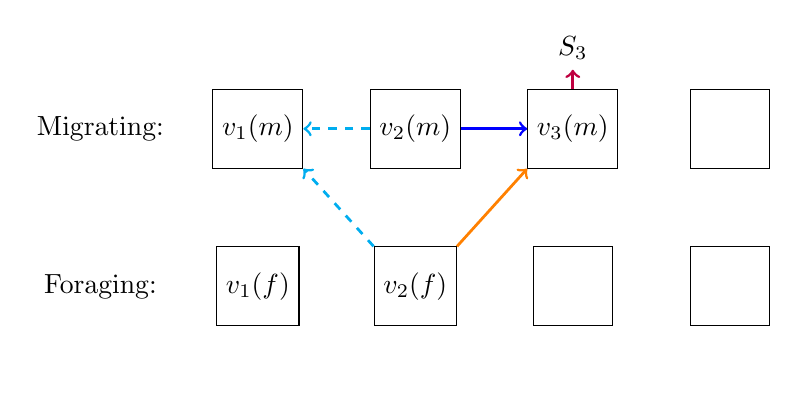
\begin{tikzpicture}[node distance=2cm, block/.style={draw, minimum width=1cm, minimum height=1cm}]

  % First row
  \node[block] (A1) {$v_1(m)$};
  \node[block, right of=A1] (A2) {$v_2(m)$};
  \node[block, right of=A2] (A3) {$v_3(m)$};
  \node[block, right of=A3] (A4) {};

  % Second row
  \node[block, below of=A1] (B1) {$v_1(f)$};
  \node[block, right of=B1] (B2) {$v_2(f)$};
  \node[block, right of=B2] (B3) {};
  \node[block, right of=B3] (B4) {};

  % Labels
  \node[coordinate, left of=A1] (J1) {};
  \node[] at (J1) {Migrating:};
  \node[coordinate, left of=B1] (J2) {};
  \node[] at (J2) {Foraging:};

  % Horizontal arrows
  \draw[->, line width=1pt, opacity=0, color=blue] (A1.east) -- (A2.west);
  \draw[->, line width=1pt, opacity=1, color=cyan, dashed] (A2.west) -- (A1.east);
  \draw[->, line width=1pt, opacity=1, color=blue] (A2.east) -- (A3.west);
  \draw[->, line width=1pt, opacity=0, color=orange] (B1.east) -- (B2.west);
  \draw[->, line width=1pt, opacity=0] (B2.east) -- (B3.west);
  \draw[->, line width=1pt, opacity=0] (B3.east) -- (B4.west);

  % Back-pointers
  

  % diagonal to blocks
  \draw[->, line width=1pt, opacity=1, color=cyan, dashed] (B2.north west) -- (A1.south east);
  \draw[->, line width=1pt, opacity=0] (A2.south east) -- (B3.north);
  \draw[->, line width=1pt, opacity=0] (A3.south east) -- (B4.north);
  \draw[->, line width=1pt, opacity=0, color=orange] (B1.north east) -- (A2.south west);
  \draw[->, line width=1pt, opacity=1, color=orange] (B2.north east) -- (A3.south west);
  \draw[->, line width=1pt, opacity=0] (B3.north east) -- (A4.south);

  \node[coordinate, above of=A1, yshift=-1.25cm] (G1) {};
  \node[above] at (G1) {};
  \node[coordinate, above of=A2, yshift=-1.25cm] (G2) {};
  \node[above] at (G2) {};
  \node[coordinate, above of=A3, yshift=-1.25cm] (G3) {};
  \node[above] at (G3) {$S_3$};
  \node[coordinate, above of=A4, yshift=-1.25cm] (G4) {};
  \node[above] at (G4) {};
  \node[coordinate, below of=B1, yshift=1.25cm] (H1) {};
  \node[below] at (H1) {};
  \node[coordinate, below of=B2, yshift=1.25cm] (H2) {};
  \node[below] at (H2) {};
  \node[coordinate, below of=B3, yshift=1.25cm] (H3) {};
  \node[below] at (H3) {};
  \node[coordinate, below of=B4, yshift=1.25cm] (H4) {};
  \node[below] at (H4) {};

  % vertical arrow
  \draw[->, line width=1pt, opacity=1, color=purple] (A3.north) -- (G3.south);

\end{tikzpicture}
\end{center}


\begin{equation*}
\begin{aligned}
    v_3(m) = \max\{&\textcolor{blue}{v_2(m) p(X_3=m | X_2=m)}, \textcolor{orange}{v_2(f) p(X_3=m | X_2=f)} \} \times\\
    &\textcolor{purple}{p(S_3|X_3=m)}.
\end{aligned}
\end{equation*}
    
\end{frame}

\begin{frame}
\frametitle{Viterbi in action}
\begin{center}
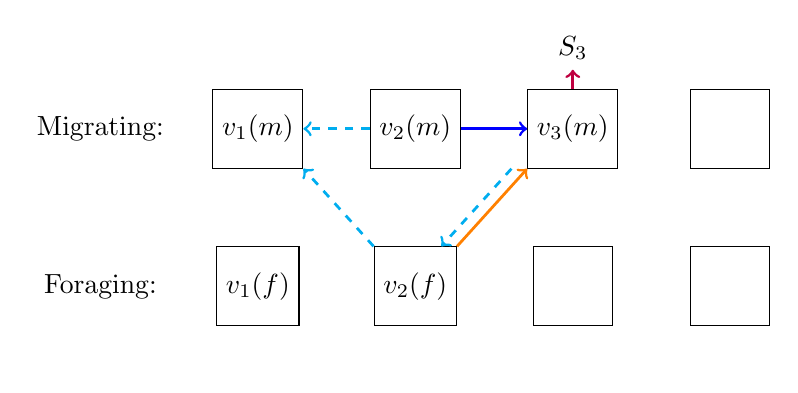
\begin{tikzpicture}[node distance=2cm, block/.style={draw, minimum width=1cm, minimum height=1cm}]

  % First row
  \node[block] (A1) {$v_1(m)$};
  \node[block, right of=A1] (A2) {$v_2(m)$};
  \node[block, right of=A2] (A3) {$v_3(m)$};
  \node[block, right of=A3] (A4) {};

  % Second row
  \node[block, below of=A1] (B1) {$v_1(f)$};
  \node[block, right of=B1] (B2) {$v_2(f)$};
  \node[block, right of=B2] (B3) {};
  \node[block, right of=B3] (B4) {};

  % Labels
  \node[coordinate, left of=A1] (J1) {};
  \node[] at (J1) {Migrating:};
  \node[coordinate, left of=B1] (J2) {};
  \node[] at (J2) {Foraging:};

  % Horizontal arrows
  \draw[->, line width=1pt, opacity=0, color=blue] (A1.east) -- (A2.west);
  \draw[->, line width=1pt, opacity=1, color=cyan, dashed] (A2.west) -- (A1.east);
  \draw[->, line width=1pt, opacity=1, color=blue] (A2.east) -- (A3.west);
  \draw[->, line width=1pt, opacity=0, color=orange] (B1.east) -- (B2.west);
  \draw[->, line width=1pt, opacity=0] (B2.east) -- (B3.west);
  \draw[->, line width=1pt, opacity=0] (B3.east) -- (B4.west);

  % Back-pointers
  \draw[->, line width=1pt, opacity=1, color=cyan, dashed] ($(A3.south west)+(-0.2cm,0cm)$) -- ($(B2.north east)+(-0.2cm,0cm)$);

  % diagonal to blocks
  \draw[->, line width=1pt, opacity=1, color=cyan, dashed] (B2.north west) -- (A1.south east);
  \draw[->, line width=1pt, opacity=0] (A2.south east) -- (B3.north);
  \draw[->, line width=1pt, opacity=0] (A3.south east) -- (B4.north);
  \draw[->, line width=1pt, opacity=0, color=orange] (B1.north east) -- (A2.south west);
  \draw[->, line width=1pt, opacity=1, color=orange] (B2.north east) -- (A3.south west);
  \draw[->, line width=1pt, opacity=0] (B3.north east) -- (A4.south);

  \node[coordinate, above of=A1, yshift=-1.25cm] (G1) {};
  \node[above] at (G1) {};
  \node[coordinate, above of=A2, yshift=-1.25cm] (G2) {};
  \node[above] at (G2) {};
  \node[coordinate, above of=A3, yshift=-1.25cm] (G3) {};
  \node[above] at (G3) {$S_3$};
  \node[coordinate, above of=A4, yshift=-1.25cm] (G4) {};
  \node[above] at (G4) {};
  \node[coordinate, below of=B1, yshift=1.25cm] (H1) {};
  \node[below] at (H1) {};
  \node[coordinate, below of=B2, yshift=1.25cm] (H2) {};
  \node[below] at (H2) {};
  \node[coordinate, below of=B3, yshift=1.25cm] (H3) {};
  \node[below] at (H3) {};
  \node[coordinate, below of=B4, yshift=1.25cm] (H4) {};
  \node[below] at (H4) {};

  % vertical arrow
  \draw[->, line width=1pt, opacity=1, color=purple] (A3.north) -- (G3.south);

\end{tikzpicture}
\end{center}

\begin{equation*}
    \text{if } \textcolor{orange}{v_2(f) p(X_3=m | X_2=f)} > \textcolor{blue}{v_2(m) p(X_3=m | X_2=m)}
\end{equation*}
    
\end{frame}

\begin{frame}
\frametitle{Viterbi in action}
\begin{center}
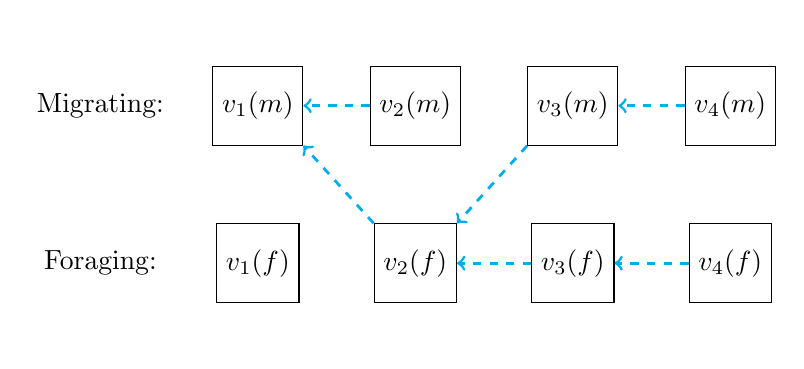
\begin{tikzpicture}[node distance=2cm, block/.style={draw, minimum width=1cm, minimum height=1cm}]

  % First row
  \node[block] (A1) {$v_1(m)$};
  \node[block, right of=A1] (A2) {$v_2(m)$};
  \node[block, right of=A2] (A3) {$v_3(m)$};
  \node[block, right of=A3] (A4) {$v_4(m)$};

  % Second row
  \node[block, below of=A1] (B1) {$v_1(f)$};
  \node[block, right of=B1] (B2) {$v_2(f)$};
  \node[block, right of=B2] (B3) {$v_3(f)$};
  \node[block, right of=B3] (B4) {$v_4(f)$};

  % Labels
  \node[coordinate, left of=A1] (J1) {};
  \node[] at (J1) {Migrating:};
  \node[coordinate, left of=B1] (J2) {};
  \node[] at (J2) {Foraging:};

  % Horizontal arrows
  \draw[->, line width=1pt, opacity=0, color=blue] (A1.east) -- (A2.west);
  \draw[->, line width=1pt, opacity=1, color=cyan, dashed] (A2.west) -- (A1.east);
  \draw[->, line width=1pt, opacity=0, color=blue] (A2.east) -- (A3.west);
  \draw[->, line width=1pt, opacity=1, color=cyan, dashed] (A4.west) -- (A3.east);
  \draw[->, line width=1pt, opacity=0, color=orange] (B1.east) -- (B2.west);
  \draw[->, line width=1pt, opacity=1, color=cyan, dashed] (B3.west) -- (B2.east);
  \draw[->, line width=1pt, opacity=1, color=cyan, dashed] (B4.west) -- (B3.east);

  % diagonal to blocks
  \draw[->, line width=1pt, opacity=1, color=cyan, dashed] (B2.north west) -- (A1.south east);
  \draw[->, line width=1pt, opacity=0] (A2.south east) -- (B3.north);
  \draw[->, line width=1pt, opacity=0] (A3.south east) -- (B4.north);
  \draw[->, line width=1pt, opacity=0, color=orange] (B1.north east) -- (A2.south west);
  \draw[->, line width=1pt, opacity=1, color=cyan, dashed] (A3.south west) -- (B2.north east);
  \draw[->, line width=1pt, opacity=0] (B3.north east) -- (A4.south);

  \node[coordinate, above of=A1, yshift=-1.25cm] (G1) {};
  \node[above] at (G1) {};
  \node[coordinate, above of=A2, yshift=-1.25cm] (G2) {};
  \node[above] at (G2) {};
  \node[coordinate, above of=A3, yshift=-1.25cm] (G3) {};
  \node[above] at (G3) {};
  \node[coordinate, above of=A4, yshift=-1.25cm] (G4) {};
  \node[above] at (G4) {};
  \node[coordinate, below of=B1, yshift=1.25cm] (H1) {};
  \node[below] at (H1) {};
  \node[coordinate, below of=B2, yshift=1.25cm] (H2) {};
  \node[below] at (H2) {};
  \node[coordinate, below of=B3, yshift=1.25cm] (H3) {};
  \node[below] at (H3) {};
  \node[coordinate, below of=B4, yshift=1.25cm] (H4) {};
  \node[below] at (H4) {};


\end{tikzpicture}
\end{center}
    
\end{frame}

\begin{frame}
\frametitle{Viterbi in action}
\begin{center}
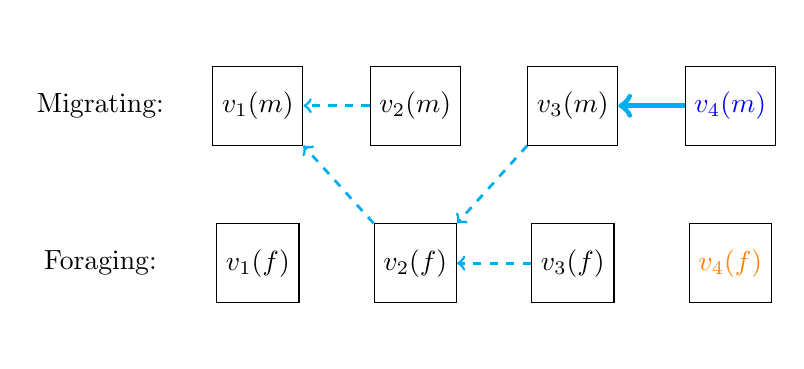
\begin{tikzpicture}[node distance=2cm, block/.style={draw, minimum width=1cm, minimum height=1cm}]

  % First row
  \node[block] (A1) {$v_1(m)$};
  \node[block, right of=A1] (A2) {$v_2(m)$};
  \node[block, right of=A2] (A3) {$v_3(m)$};
  \node[block, right of=A3] (A4) {$\textcolor{blue}{v_4(m)}$};

  % Second row
  \node[block, below of=A1] (B1) {$v_1(f)$};
  \node[block, right of=B1] (B2) {$v_2(f)$};
  \node[block, right of=B2] (B3) {$v_3(f)$};
  \node[block, right of=B3] (B4) {$\textcolor{orange}{v_4(f)}$};

  % Labels
  \node[coordinate, left of=A1] (J1) {};
  \node[] at (J1) {Migrating:};
  \node[coordinate, left of=B1] (J2) {};
  \node[] at (J2) {Foraging:};

  % Horizontal arrows
  \draw[->, line width=1pt, opacity=0, color=blue] (A1.east) -- (A2.west);
  \draw[->, line width=1pt, opacity=1, color=cyan, dashed] (A2.west) -- (A1.east);
  \draw[->, line width=1pt, opacity=0, color=blue] (A2.east) -- (A3.west);
  \draw[->, line width=2pt, opacity=1, color=cyan] (A4.west) -- (A3.east);
  \draw[->, line width=1pt, opacity=0, color=orange] (B1.east) -- (B2.west);
  \draw[->, line width=1pt, opacity=1, color=cyan, dashed] (B3.west) -- (B2.east);
  \draw[->, line width=1pt, opacity=0, color=cyan, dashed] (B4.west) -- (B3.east);

  % diagonal to blocks
  \draw[->, line width=1pt, opacity=1, color=cyan, dashed] (B2.north west) -- (A1.south east);
  \draw[->, line width=1pt, opacity=0] (A2.south east) -- (B3.north);
  \draw[->, line width=1pt, opacity=0] (A3.south east) -- (B4.north);
  \draw[->, line width=1pt, opacity=0, color=orange] (B1.north east) -- (A2.south west);
  \draw[->, line width=1pt, opacity=1, color=cyan, dashed] (A3.south west) -- (B2.north east);
  \draw[->, line width=1pt, opacity=0] (B3.north east) -- (A4.south);

  \node[coordinate, above of=A1, yshift=-1.25cm] (G1) {};
  \node[above] at (G1) {};
  \node[coordinate, above of=A2, yshift=-1.25cm] (G2) {};
  \node[above] at (G2) {};
  \node[coordinate, above of=A3, yshift=-1.25cm] (G3) {};
  \node[above] at (G3) {};
  \node[coordinate, above of=A4, yshift=-1.25cm] (G4) {};
  \node[above] at (G4) {};
  \node[coordinate, below of=B1, yshift=1.25cm] (H1) {};
  \node[below] at (H1) {};
  \node[coordinate, below of=B2, yshift=1.25cm] (H2) {};
  \node[below] at (H2) {};
  \node[coordinate, below of=B3, yshift=1.25cm] (H3) {};
  \node[below] at (H3) {};
  \node[coordinate, below of=B4, yshift=1.25cm] (H4) {};
  \node[below] at (H4) {};


\end{tikzpicture}
\end{center}

\begin{equation*}
    \text{if } \textcolor{blue}{v_4(m)} > \textcolor{orange}{v_4(f)}
\end{equation*}
    
\end{frame}

\begin{frame}
\frametitle{Viterbi in action}
\begin{center}
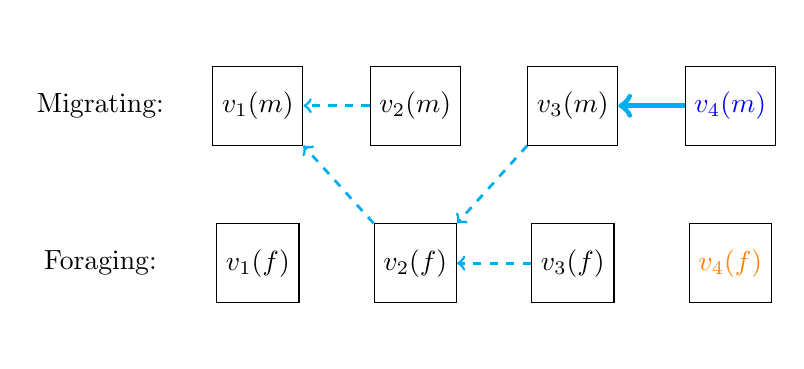
\begin{tikzpicture}[node distance=2cm, block/.style={draw, minimum width=1cm, minimum height=1cm}]

  % First row
  \node[block] (A1) {$v_1(m)$};
  \node[block, right of=A1] (A2) {$v_2(m)$};
  \node[block, right of=A2] (A3) {$v_3(m)$};
  \node[block, right of=A3] (A4) {$\textcolor{blue}{v_4(m)}$};

  % Second row
  \node[block, below of=A1] (B1) {$v_1(f)$};
  \node[block, right of=B1] (B2) {$v_2(f)$};
  \node[block, right of=B2] (B3) {$v_3(f)$};
  \node[block, right of=B3] (B4) {$\textcolor{orange}{v_4(f)}$};

  % Labels
  \node[coordinate, left of=A1] (J1) {};
  \node[] at (J1) {Migrating:};
  \node[coordinate, left of=B1] (J2) {};
  \node[] at (J2) {Foraging:};

  % Horizontal arrows
  \draw[->, line width=1pt, opacity=0, color=blue] (A1.east) -- (A2.west);
  \draw[->, line width=1pt, opacity=1, color=cyan, dashed] (A2.west) -- (A1.east);
  \draw[->, line width=1pt, opacity=0, color=blue] (A2.east) -- (A3.west);
  \draw[->, line width=2pt, opacity=1, color=cyan] (A4.west) -- (A3.east);
  \draw[->, line width=1pt, opacity=0, color=orange] (B1.east) -- (B2.west);
  \draw[->, line width=1pt, opacity=1, color=cyan, dashed] (B3.west) -- (B2.east);
  \draw[->, line width=1pt, opacity=0, color=cyan, dashed] (B4.west) -- (B3.east);

  % diagonal to blocks
  \draw[->, line width=1pt, opacity=1, color=cyan, dashed] (B2.north west) -- (A1.south east);
  \draw[->, line width=1pt, opacity=0] (A2.south east) -- (B3.north);
  \draw[->, line width=1pt, opacity=0] (A3.south east) -- (B4.north);
  \draw[->, line width=1pt, opacity=0, color=orange] (B1.north east) -- (A2.south west);
  \draw[->, line width=1pt, opacity=1, color=cyan, dashed] (A3.south west) -- (B2.north east);
  \draw[->, line width=1pt, opacity=0] (B3.north east) -- (A4.south);

  \node[coordinate, above of=A1, yshift=-1.25cm] (G1) {};
  \node[above] at (G1) {};
  \node[coordinate, above of=A2, yshift=-1.25cm] (G2) {};
  \node[above] at (G2) {};
  \node[coordinate, above of=A3, yshift=-1.25cm] (G3) {};
  \node[above] at (G3) {};
  \node[coordinate, above of=A4, yshift=-1.25cm] (G4) {};
  \node[above] at (G4) {};
  \node[coordinate, below of=B1, yshift=1.25cm] (H1) {};
  \node[below] at (H1) {};
  \node[coordinate, below of=B2, yshift=1.25cm] (H2) {};
  \node[below] at (H2) {};
  \node[coordinate, below of=B3, yshift=1.25cm] (H3) {};
  \node[below] at (H3) {};
  \node[coordinate, below of=B4, yshift=1.25cm] (H4) {};
  \node[below] at (H4) {};


\end{tikzpicture}
\end{center}

\begin{equation*}
    \text{if } \textcolor{blue}{v_4(m)} > \textcolor{orange}{v_4(f)}
\end{equation*}
    
\end{frame}

\begin{frame}
\frametitle{Viterbi in action}
\begin{center}
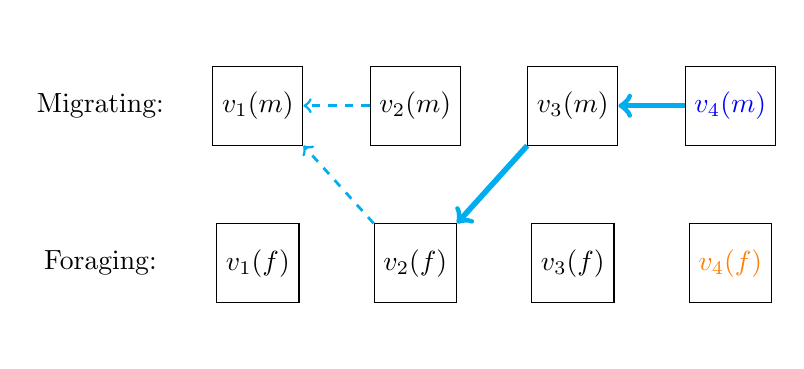
\begin{tikzpicture}[node distance=2cm, block/.style={draw, minimum width=1cm, minimum height=1cm}]

  % First row
  \node[block] (A1) {$v_1(m)$};
  \node[block, right of=A1] (A2) {$v_2(m)$};
  \node[block, right of=A2] (A3) {$v_3(m)$};
  \node[block, right of=A3] (A4) {$\textcolor{blue}{v_4(m)}$};

  % Second row
  \node[block, below of=A1] (B1) {$v_1(f)$};
  \node[block, right of=B1] (B2) {$v_2(f)$};
  \node[block, right of=B2] (B3) {$v_3(f)$};
  \node[block, right of=B3] (B4) {$\textcolor{orange}{v_4(f)}$};

  % Labels
  \node[coordinate, left of=A1] (J1) {};
  \node[] at (J1) {Migrating:};
  \node[coordinate, left of=B1] (J2) {};
  \node[] at (J2) {Foraging:};

  % Horizontal arrows
  \draw[->, line width=1pt, opacity=0, color=blue] (A1.east) -- (A2.west);
  \draw[->, line width=1pt, opacity=1, color=cyan, dashed] (A2.west) -- (A1.east);
  \draw[->, line width=1pt, opacity=0, color=blue] (A2.east) -- (A3.west);
  \draw[->, line width=2pt, opacity=1, color=cyan] (A4.west) -- (A3.east);
  \draw[->, line width=1pt, opacity=0, color=orange] (B1.east) -- (B2.west);
  \draw[->, line width=1pt, opacity=0, color=cyan, dashed] (B3.west) -- (B2.east);
  \draw[->, line width=1pt, opacity=0, color=cyan, dashed] (B4.west) -- (B3.east);

  % diagonal to blocks
  \draw[->, line width=1pt, opacity=1, color=cyan, dashed] (B2.north west) -- (A1.south east);
  \draw[->, line width=1pt, opacity=0] (A2.south east) -- (B3.north);
  \draw[->, line width=1pt, opacity=0] (A3.south east) -- (B4.north);
  \draw[->, line width=1pt, opacity=0, color=orange] (B1.north east) -- (A2.south west);
  \draw[->, line width=2pt, opacity=1, color=cyan] (A3.south west) -- (B2.north east);
  \draw[->, line width=1pt, opacity=0] (B3.north east) -- (A4.south);

  \node[coordinate, above of=A1, yshift=-1.25cm] (G1) {};
  \node[above] at (G1) {};
  \node[coordinate, above of=A2, yshift=-1.25cm] (G2) {};
  \node[above] at (G2) {};
  \node[coordinate, above of=A3, yshift=-1.25cm] (G3) {};
  \node[above] at (G3) {};
  \node[coordinate, above of=A4, yshift=-1.25cm] (G4) {};
  \node[above] at (G4) {};
  \node[coordinate, below of=B1, yshift=1.25cm] (H1) {};
  \node[below] at (H1) {};
  \node[coordinate, below of=B2, yshift=1.25cm] (H2) {};
  \node[below] at (H2) {};
  \node[coordinate, below of=B3, yshift=1.25cm] (H3) {};
  \node[below] at (H3) {};
  \node[coordinate, below of=B4, yshift=1.25cm] (H4) {};
  \node[below] at (H4) {};


\end{tikzpicture}
\end{center}

\begin{equation*}
    \text{if } \textcolor{blue}{v_4(m)} > \textcolor{orange}{v_4(f)}
\end{equation*}
    
\end{frame}

\begin{frame}
\frametitle{Viterbi in action}
\begin{center}
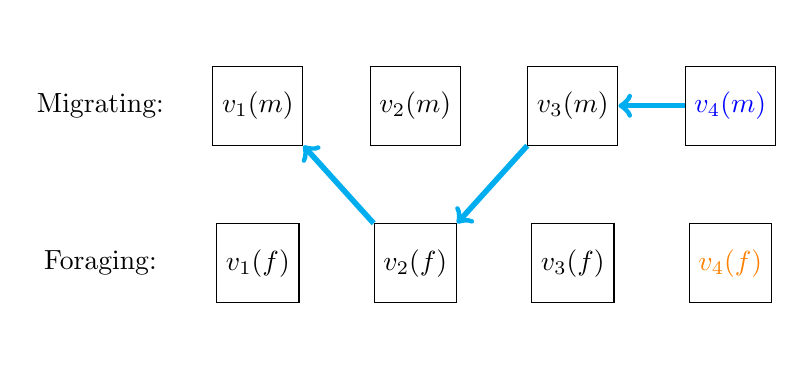
\begin{tikzpicture}[node distance=2cm, block/.style={draw, minimum width=1cm, minimum height=1cm}]

  % First row
  \node[block] (A1) {$v_1(m)$};
  \node[block, right of=A1] (A2) {$v_2(m)$};
  \node[block, right of=A2] (A3) {$v_3(m)$};
  \node[block, right of=A3] (A4) {$\textcolor{blue}{v_4(m)}$};

  % Second row
  \node[block, below of=A1] (B1) {$v_1(f)$};
  \node[block, right of=B1] (B2) {$v_2(f)$};
  \node[block, right of=B2] (B3) {$v_3(f)$};
  \node[block, right of=B3] (B4) {$\textcolor{orange}{v_4(f)}$};

  % Labels
  \node[coordinate, left of=A1] (J1) {};
  \node[] at (J1) {Migrating:};
  \node[coordinate, left of=B1] (J2) {};
  \node[] at (J2) {Foraging:};

  % Horizontal arrows
  \draw[->, line width=1pt, opacity=0, color=blue] (A1.east) -- (A2.west);
  \draw[->, line width=1pt, opacity=0, color=cyan, dashed] (A2.west) -- (A1.east);
  \draw[->, line width=1pt, opacity=0, color=blue] (A2.east) -- (A3.west);
  \draw[->, line width=2pt, opacity=1, color=cyan] (A4.west) -- (A3.east);
  \draw[->, line width=1pt, opacity=0, color=orange] (B1.east) -- (B2.west);
  \draw[->, line width=1pt, opacity=0, color=cyan, dashed] (B3.west) -- (B2.east);
  \draw[->, line width=1pt, opacity=0, color=cyan, dashed] (B4.west) -- (B3.east);

  % diagonal to blocks
  \draw[->, line width=2pt, opacity=1, color=cyan] (B2.north west) -- (A1.south east);
  \draw[->, line width=1pt, opacity=0] (A2.south east) -- (B3.north);
  \draw[->, line width=1pt, opacity=0] (A3.south east) -- (B4.north);
  \draw[->, line width=1pt, opacity=0, color=orange] (B1.north east) -- (A2.south west);
  \draw[->, line width=2pt, opacity=1, color=cyan] (A3.south west) -- (B2.north east);
  \draw[->, line width=1pt, opacity=0] (B3.north east) -- (A4.south);

  \node[coordinate, above of=A1, yshift=-1.25cm] (G1) {};
  \node[above] at (G1) {};
  \node[coordinate, above of=A2, yshift=-1.25cm] (G2) {};
  \node[above] at (G2) {};
  \node[coordinate, above of=A3, yshift=-1.25cm] (G3) {};
  \node[above] at (G3) {};
  \node[coordinate, above of=A4, yshift=-1.25cm] (G4) {};
  \node[above] at (G4) {};
  \node[coordinate, below of=B1, yshift=1.25cm] (H1) {};
  \node[below] at (H1) {};
  \node[coordinate, below of=B2, yshift=1.25cm] (H2) {};
  \node[below] at (H2) {};
  \node[coordinate, below of=B3, yshift=1.25cm] (H3) {};
  \node[below] at (H3) {};
  \node[coordinate, below of=B4, yshift=1.25cm] (H4) {};
  \node[below] at (H4) {};


\end{tikzpicture}
\end{center}

\begin{equation*}
    \text{if } \textcolor{blue}{v_4(m)} > \textcolor{orange}{v_4(f)}
\end{equation*}
    
\end{frame}

\begin{frame}
\frametitle{Viterbi in action}
\begin{center}
\begin{tikzpicture}[node distance=2cm, block/.style={draw, minimum width=1cm, minimum height=1cm}]

  % First row
  \node[block] (A1) {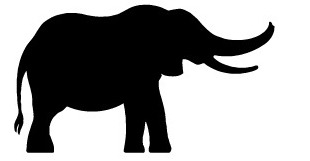
\includegraphics[width=1cm]{figures/elephant.jpg}};
  \node[block, right of=A1] (A2) {};
  \node[block, right of=A2] (A3) {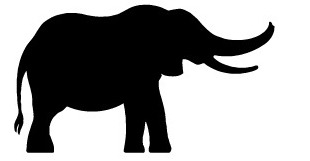
\includegraphics[width=1cm]{figures/elephant.jpg}};
  \node[block, right of=A3] (A4) {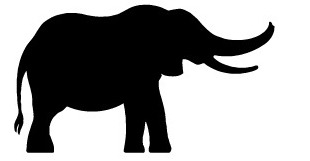
\includegraphics[width=1cm]{figures/elephant.jpg}};

  % Second row
  \node[block, below of=A1] (B1) {};
  \node[block, right of=B1] (B2) {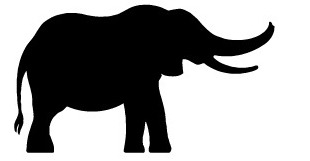
\includegraphics[width=1cm]{figures/elephant.jpg}};
  \node[block, right of=B2] (B3) {};
  \node[block, right of=B3] (B4) {};

  % Labels
  \node[coordinate, left of=A1] (J1) {};
  \node[] at (J1) {Migrating:};
  \node[coordinate, left of=B1] (J2) {};
  \node[] at (J2) {Foraging:};

  % Horizontal arrows
  \draw[->, line width=1pt, opacity=0, color=blue] (A1.east) -- (A2.west);
  \draw[->, line width=1pt, opacity=0, color=cyan, dashed] (A2.west) -- (A1.east);
  \draw[->, line width=1pt, opacity=0, color=blue] (A2.east) -- (A3.west);
  \draw[->, line width=2pt, opacity=1, color=cyan]  (A3.east) -- (A4.west);
  \draw[->, line width=1pt, opacity=0, color=orange] (B1.east) -- (B2.west);
  \draw[->, line width=1pt, opacity=0, color=cyan, dashed] (B3.west) -- (B2.east);
  \draw[->, line width=1pt, opacity=0, color=cyan, dashed] (B4.west) -- (B3.east);

  % diagonal to blocks
  \draw[->, line width=2pt, opacity=1, color=cyan] (A1.south east) -- (B2.north west);
  \draw[->, line width=1pt, opacity=0] (A2.south east) -- (B3.north);
  \draw[->, line width=1pt, opacity=0] (A3.south east) -- (B4.north);
  \draw[->, line width=1pt, opacity=0, color=orange] (B1.north east) -- (A2.south west);
  \draw[->, line width=2pt, opacity=1, color=cyan] (B2.north east) -- (A3.south west);
  \draw[->, line width=1pt, opacity=0] (B3.north east) -- (A4.south);

  \node[coordinate, above of=A1, yshift=-1.25cm] (G1) {};
  \node[above] at (G1) {};
  \node[coordinate, above of=A2, yshift=-1.25cm] (G2) {};
  \node[above] at (G2) {};
  \node[coordinate, above of=A3, yshift=-1.25cm] (G3) {};
  \node[above] at (G3) {};
  \node[coordinate, above of=A4, yshift=-1.25cm] (G4) {};
  \node[above] at (G4) {};
  \node[coordinate, below of=B1, yshift=1.25cm] (H1) {};
  \node[below] at (H1) {};
  \node[coordinate, below of=B2, yshift=1.25cm] (H2) {};
  \node[below] at (H2) {};
  \node[coordinate, below of=B3, yshift=1.25cm] (H3) {};
  \node[below] at (H3) {};
  \node[coordinate, below of=B4, yshift=1.25cm] (H4) {};
  \node[below] at (H4) {};


\end{tikzpicture}
\end{center}

\begin{equation*}
    \text{if } \textcolor{blue}{v_4(m)} > \textcolor{orange}{v_4(f)}
\end{equation*}
    
\end{frame}

\begin{frame}
\frametitle{Bayesian inference of HMMs}
    
\end{frame}

\begin{frame}
\frametitle{Elephants revisited}

Restate problem.
    
\end{frame}

\begin{frame}
\frametitle{Reducing degrees of freedom in HMM}

Did we use any other info but speed?
    
\end{frame}

\end{document}